\documentclass[twoside]{report}
\usepackage[utf8]{inputenc}
\usepackage[english]{babel}
\usepackage[numbers]{natbib}
\usepackage{amsthm}
\usepackage{tkz-fct} 
\usepackage{thmtools}
\usepackage[margin=1in]{geometry}
\usepackage{amsmath,amssymb}
\usepackage{multicol}
\usepackage{graphicx}
\usepackage{tikz}
\usepackage{listings}
\usetikzlibrary{positioning} 
\usetikzlibrary{calc,patterns,angles,quotes}
\usetikzlibrary{calc,arrows, arrows.meta}
\tikzset{
  arrow/.pic={\path[tips,every arrow/.try,->,>=#1] (0,0) -- +(.1pt,0);},
  pics/arrow/.default={triangle 90}
}
\usepackage{pgfplots}% also loads graphicx
\pgfplotsset{compat=1.11} %width=10cm,
\usetikzlibrary{backgrounds}
\usepackage{siunitx}
\sisetup{per-mode=fraction} %,fraction-function = \nicefrac}
\DeclareSIUnit{\gallon}{gal}
\usepackage{fancyhdr}
\usepackage{pst-node}
\psset{nodesep=2pt,linearc=2pt,arrows=->,linecolor=blue,arrowinset=0}
\def\lbl#1{\ncput*{\text{\tiny #1}}}
\usepackage{xcolor}
\usepackage{tcolorbox}
\usepackage{lmodern}
\usepackage{relsize}
\newcommand{\highlight}[1]{%
  \colorbox{red!50}{$\displaystyle#1$}}
\usepackage{url}
\usepackage{cancel}
\usepackage{mwe}
\usepackage{caption}
\usepackage{float}
\usepackage{setspace}
\usepackage{hyperref}
\usepackage{subcaption}
\usepackage{varwidth}
\usepackage{todonotes}
% set the arrows as stealth fighters (personal preference)
\tikzset{>=stealth}
\captionsetup[figure]{labelfont={bf},name={Figure},labelsep=period}

\declaretheoremstyle[
  spaceabove=6pt, spacebelow=6pt,
  headfont={\color{blue}\fontfamily{cmss}\selectfont\bfseries},
  notefont=\fontfamily{cmss}\selectfont\bfseries, notebraces={(}{)},
bodyfont=\fontfamily{cmss}\selectfont\itshape,
  postheadspace=1em,
]{mystyle}
\declaretheorem[style=mystyle,numbered=no]{definition}
\declaretheorem[style=mystyle,numbered=no]{lemma}

\declaretheoremstyle[
  spaceabove=6pt, spacebelow=6pt,
  headfont={\color{black} \fontfamily{cmss}\selectfont\bfseries},
  notefont=\fontfamily{cmss}\selectfont\bfseries, notebraces={(}{)},
bodyfont=\fontfamily{cmss}\selectfont,
  postheadspace=1em,
  qed=$\triangle$
]{mystyle2}
\declaretheorem[style=mystyle2,numbered=no]{remark}

\declaretheoremstyle[
  spaceabove=6pt, spacebelow=6pt,
  headfont={\color{orange} \fontfamily{cmss}\selectfont\bfseries},
  notefont=\fontfamily{cmss}\selectfont\bfseries, notebraces={(}{)},
bodyfont=\fontfamily{cmss}\selectfont,
  postheadspace=1em,
  qed=$\triangle$
]{mystyle3}
\declaretheorem[style=mystyle3,numbered=no]{example}

\declaretheoremstyle[
  spaceabove=6pt, spacebelow=6pt,
  headfont={\color{blue} \fontfamily{cmss}\selectfont\bfseries},
  notefont=\fontfamily{cmss}\selectfont\bfseries, notebraces={(}{)},
  bodyfont=\fontfamily{cmss}\selectfont\itshape,
  postheadspace=1em,
  qed=
]{mystyle4}
\declaretheorem[style=mystyle4,numbered=no]{law}

\declaretheoremstyle[
  spaceabove=6pt, spacebelow=6pt,
  headfont={\color{blue} \fontfamily{cmss}\selectfont\bfseries},
  notefont=\fontfamily{cmss}\selectfont\bfseries, notebraces={(}{)},
bodyfont=\fontfamily{cmss}\selectfont,
  postheadspace=1em,
  qed=
]{mystyle5}
\declaretheorem[style=mystyle5,numbered=no]{strategy}

\declaretheoremstyle[
  spaceabove=6pt, spacebelow=6pt,
  headfont={\color{blue} \fontfamily{cmss}\selectfont\bfseries},
  notefont=\fontfamily{cmss}\selectfont\bfseries, notebraces={(}{)},
bodyfont=\fontfamily{cmss}\selectfont\itshape,
  postheadspace=1em,
  qed=
]{mystyle6}
\declaretheorem[style=mystyle6,numbered=no]{theorem}


\renewcommand{\qedsymbol}{\rule{0.7em}{0.7em}}
\renewenvironment{proof}{{\bfseries \fontfamily{cmss} \scshape Proof:}}



\newcommand{\reporttitle}{}
\newcommand{\reportauthor}{Kai Cooper}
\newcommand{\reportsecondauthor}{Yehao Liu}
\newcommand{\reportthirdauthor}{Yacine Trad}
\newcommand{\reportfourthauthor}{ZachHFT}
\newcommand{\reportfifthauthor}{}
\newcommand{\supervisor}{Dr. Mehdi Gholam \\ Celia Garcia Pareja}

\date{June 2021}

\renewcommand{\chaptername}{Part}
\newcommand{\lap}{\nabla^2}
\newcommand{\dif}[1]{\text{d}#1}

\newcommand{\code}{\texttt}
\renewcommand{\floatpagefraction}{.8}

\definecolor{fcolor}{RGB}{0,255,255}




\begin{document}
\begin{spacing}{1}
% Last modification: 2015-08-17 (Marc Deisenroth)
\begin{titlepage}

\newcommand{\HRule}{\rule{\linewidth}{0.5mm}} % Defines a new command for the horizontal lines, change thickness here


%----------------------------------------------------------------------------------------
%	LOGO SECTION
%----------------------------------------------------------------------------------------

%\includegraphics[width = 4cm]{}\\[0.5cm] 

\center % Center remainder of the page

%----------------------------------------------------------------------------------------
%	HEADING SECTIONS
%----------------------------------------------------------------------------------------

\textsc{\Large École Polytéchnique Fédérale de Lausanne}\\[0.5cm] 
\textsc{\large Department of Mathematics}\\[0.5cm] 

%----------------------------------------------------------------------------------------
%	TITLE SECTION
%----------------------------------------------------------------------------------------

\HRule \\[0.4cm]
{ \huge \bfseries Discovery and Assessment of optimal cryptocurrency trading strategies \reporttitle}\\ % Title of your document
\HRule \\[1.5cm]
 
%----------------------------------------------------------------------------------------
%	AUTHOR SECTION
%----------------------------------------------------------------------------------------

\begin{minipage}{0.4\textwidth}
\begin{flushleft} \large
\emph{Authors:}\\
\reportauthor\\ % Your name
\reportsecondauthor\\
\reportthirdauthor\\
\reportfourthauthor\\
\reportfifthauthor
\end{flushleft}
\end{minipage}
~
\begin{minipage}{0.4\textwidth}
\begin{flushright} \large
\emph{Supervisors:} \\
\supervisor % Supervisor's Name
\end{flushright}
\end{minipage}\\[4cm]


%----------------------------------------------------------------------------------------
%	FOOTER & DATE SECTION
%----------------------------------------------------------------------------------------
\vfill % Fill the rest of the page with whitespace

\makeatletter
\@date
\makeatother


\end{titlepage}
\fontfamily{cmss}\selectfont
\tableofcontents



\chapter{Introduction}

\section{Background and scope}
A cryptocurrency is a tradable digital asset or digital form of money, built on blockchain technology that only exists online. Examples include Bitcoin, Ethereum and Dogecoin. Since its inception in 2008, its popularity has done nothing but grow, leisurely at first, but its popularity has somewhat exploded in recent years. Cryptocurrencies are attractive to many because they are accessible to all, unlike the traditional stock market (until recently). For this reason, their prices are highly susceptible to a variety of factors such as news and social media, much like that of a traditional stock market although perhaps even more sensitive due to the nonexistent perspective of exclusivity -- for example, prices could change due to a trend on Instagram, instead of the more high-level and obscure knowledge of a scandalous exodus of a large company CEO. The aim of this project is to find macro-scale factors which drive fluctuations in cryptocurrency prices and to leverage them in developing profit generating trading strategies. 

Let us breifly offer some technical backgorund. When faced with a given cryptocurrency, what we see on a graph of the \textbf{price} of a currency is the value of a single \textbf{token}. The value of a token is equal to the market cap (total value of the network; denoted MC) of a currency divided by the total circulating supply (number of tokens; denoted CS). For example, Bitcoin has a circulating supply of 19 million tokens but a total supply of 21 million tokens. The difference between the circulating supply and the total supply is the amount still available to be mined, and indicates future inflation. 
\[\text{Value of a Token}\, =\frac{\text{MC}}{\text{CS}}.\]
\begin{figure}[!htbp]
    \centering
    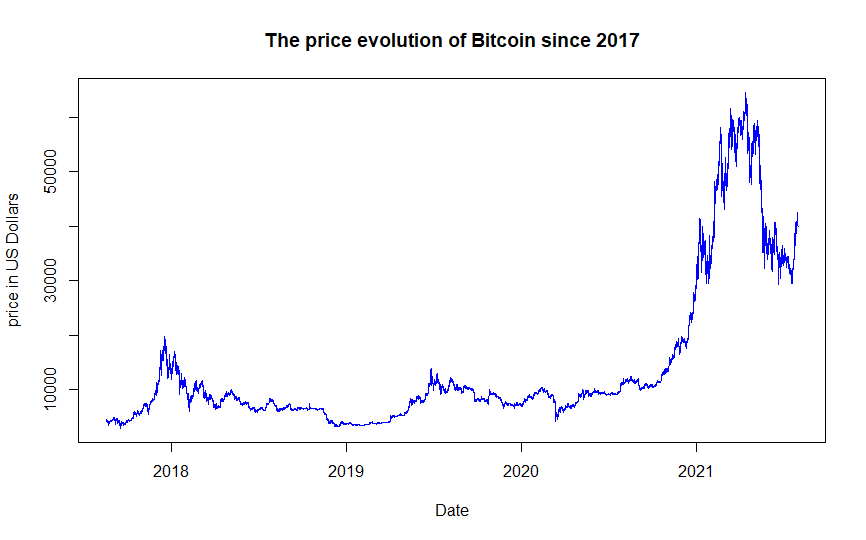
\includegraphics[scale = 0.7]{TestPlots/BTC_overview.png}
    \caption{The price chart of Bitcoin from 2017 to 2021}
    \label{BTC overall}
\end{figure}
In Figure (\ref{BTC overall}), we look at the value of this token in USD over a significant period of time. One realises that Bitcoin prices have been very volatile over the years and this feature is shared by many other cryptocurrencies. Bitcoin went from $10,000$ USD in September 2020 to over $60,000$ USD in April 2021, but also lost half of it's value from April to July 2021. Of course, not all cryptos follow the same trends simultaneously. Some might be rising while others are crashing, and the goal of crypto-trading is to ride the right wave at the right time, and jump off the ship before it sinks. That is why it is sensible to deal with pairs cryptocurrencies to explot the relationships between them.\\

\section{Aim}

The goal of this project is to proceed to the analysis of an optimal trading (buy-and-sell) strategy for the market of Cryptocurrencies. In particular, we will investigate 4 range of strategies, namely, a first general Exploratory Data Analysis which shall lead us to discover some general historical trends over the days and months of trading (e.g. Thursday is generally a bad day to trade Bitcoin with a negative log-return overall). Secondly, we will investigate how social networks influences cryptocurrencies prices, we will propose buy-and-sell strategies accordingly, and shall backtest the latter. Later on in the project we shall proceed to analysis of cryptocurrencies interactions, cycles, and trends forecasting. We wish to pick the top trending cryptocurrencies right before they actually become top-trending cryptocurrencies. We shall conclude this project with the analysis of extremes fluctuations in price. \\

Before starting our analysis, the reader should know that, unlike stock markets, the data for which are extremely onerous to acces, cryptocurrencies data are far less expensive and far more accessible. In particular, we use Binance's (a major cryptocurrency exchange platform) API to extract the historical trading prices of every exchange pair on its platform. It's API allows us to obtain the historical prices over 1 day, 1 hour, and even 1 minute period. We shall obtain open, high, low, close (OHLC) prices for the according period. The trading volume is also provided. We provide further details regarding these data in the next section. A subset of the historical data we use is available at this link: \url{https://drive.switch.ch/index.php/s/URDxQbEv8LqSkB2}.


\section{Data}
\subsection{Data extraction and processing}
The data extracted from Binance's API -- using Python to access it -- will contain price data at various time points and intervals for a chosen cryptocurrency. We remark that that we have never encountered any NA values or other seemingly out-of-place values that would need to be rejected. Indeed, so called 'out-of-place values' or any other outliers kind of value are strong indicators which require further investigations and may be relevant to dedicated algorithmic trading strategies. We absolutely do not want to remove them as we may be tempted to do in some other contexts in data science.\\

From time to time, one might find missing time periods in the extracted data. Fo example, every once in a while there is a major crash in cryptocurrencies market (i.e. prices dropping significantly). This leads to a massive amount of people trying to connect to the cryptocurrencies exchange platforms to try to sell (or buy) some cryptocurrencies.This often results in the exchange becoming unavailable, their server not being able to handle so many connections attempts at once. This explains the missing data in historical cryptocurrencies prices data (It can be for a couple of minutes up to a couple of hours). We therefore compute the time difference in days and time difference in minutes between pairs of consectives rows of data to spot any such discrepancies in the timestamp and add these to the data set. For example, in a 1-hour dataset we expect that time difference between line i and line i-1 to be 60 min, if, say, it appears to be 57 minutes, we know there was a crash that occured and therefore can decide our strategy testing programme to not consider (i.e. to pause) this very particular time period. It is a useful method to rigoursly proceed to strategy testing algorithm. 
Although, for the purposes of statistical analysis this discrepancy can be problematic. One way to circumvent this issue is to \textbf{impute} the time series, and there are software packages available to do this. For example, in section \ref{reddit} on Reddit networks, an R package called \code{imputeTS} is used to do this, with the function \code{na\_kalman} which replaces \code{NA} values in the dataset using nearby values by Kalman Smoothing \cite{KalmanFilter}. This method is one of the most recommended in the package.

\begin{figure}[H]
    \centering
    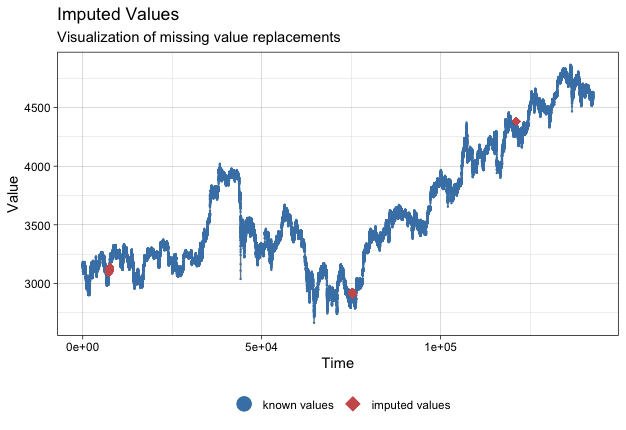
\includegraphics[width=\linewidth]{Reddit_Analysis/Price_Data_Extraction/Data/Binance_OHLC/imputed_gg_1m.png}
    \caption{Imputed values of time series. The graph is generated automatically with the function \code{ggplot\_na\_imputations} in the \code{imputeTS} package.}
    \label{fig:imputations}
\end{figure}


Going further, once an analysis is performed on a dedicated dataset (e.g. 1 hour BTC/USDT historical data), the same statistical analysis can be performed over any dataset (e.g. 1 minute ETH/CHF historical data), since the data structure (i.e. the columns, open, high, low, close) is the same.

\subsection{Data transformation}

The goal of this project is to proceed to the analysis of an optimal trading (buy-and-sell) strategy for the market of cryptocurrencies. Our analysis will be made on cryptocurrency pairs. These pairs allow us to compare costs between different cryptocurrencies. They are helpful for illustrating the relative worth of coins. For example,the question how much Bitcoin (BTC) equals in Ethereum (ETH) will be answered by the value of the pair BTC/ETH. In this report we will often be dealing with the BTC/USDT pair. USDT stands for Tether which is a stable coin in which each token is backed by a U.S Dollar.
The price of a token depends on the market cap of the currency and how many tokens are issued. Since there are hundreds of cryptocurrencies dealing with their prices can become very cumbersome and lack clarity. For that very reason, we have chosen to deal in our analysis with log-returns.
Indeed, the price of a currency is not what is of interest to us but rather it's evolution. By studying prices we would be confronted with values that don't have an intrinsic meaning, However with log returns we will have an idea of the evolution in percentages, which is way more useful. To sum it up, this allows measuring a lot of variables in a comparable metric, thus enabling evaluation of analytic relationships amongst two or more variables despite originating from price series of unequal values. 
Concretely, if we are doing our study on a currency at time $i$ which is valued at price $p_i$. The log-return for the period $t$ is:
\[
\log\left(\frac{p_i}{p_{i-t}}\right)
\]
Another important property is the additivity of the log-return. If our price at $t_1$ is $p_1$, it changes to $p_2$ at $t_2$ and move to $p_3$ at $t_3$. The log return from $t_1 $ to $t_2$ is $\log (p_2) - \log (p_1)$, the log return from $t_2 $ to $t_3$ is $\log (p_3) - \log (p_2)$. Therefore, it is clear that the log return from $t_1 $ to $t_3$ is $\log (p_3) - \log (p_1)$. This can be calculated easily. However, if we use simple return, the return should be $p_3/p_1$ instead of $p_3/p_2 + p_2/p_1$. Hence, log-return is easier to apply to real data.

\section{Exploratory data analysis}
Exploratory data analysis (EDA) is used in data analysis to analyze and investigate data sets and summarize their main characteristics. It helps determine how best to manipulate data sources to get the answers you need, making it easier to discover patterns, spot anomalies, test a hypothesis, or check assumptions.

EDA is primarily used to see what data can reveal beyond the formal modeling or hypothesis testing task and provides a provides a better understanding of data set variables and the relationships between them. It can also help determine if the statistical techniques you are considering for data analysis are appropriate. Originally developed by American mathematician John Tukey in the 1970s, EDA techniques continue to be a widely used method in the data discovery process today.

The main purpose of EDA is to help look at data before making any assumptions. It can help identify obvious errors, as well as better understand patterns within the data, detect outliers or anomalous events, find interesting relations among the variables.



\subsection{Distribution of prices and returns}

As the very many stimuli and decisions that are involved in human decisions on the market are unknown to us, it is standard to treat price trajectories on markets such as the crypto market as stochastic. Consequently, we aim to have at least an elementary understanding of how prices change and how much trading occurs at any given time in the event that this information gives us inspiration for certain trading strategies. Figure (\ref{log return box}) shows the box plot of log-return of BTC. As can be seen from the graph, the mean value of log-return changing is around 0. with the first and third quantile around $-0.02$ and $0.02$. It is worth mentioning that there are lots of outliers. This means the price changes drastically on some days. -- this could motivate the study of extremes to find profit making opportunities. 

Figure (\ref{7day rolling volume}) is about 7 days rolling average of the volume. As the average volume is different within a week (tn the weekday, there are more trades than in the weekend), we calculate the average volume of 7days to smooth the plot. From this figure, we see that the volume oscillate during our examining period. The volume sometime change drastically for a certain day. However, with the existence of up and down signals, we see there is a trend of volume increasing from the beginning of July 2017 to July 2021.


\begin{figure}[!htbp]
\centering
\begin{subfigure}{.5\textwidth}
    \centering
    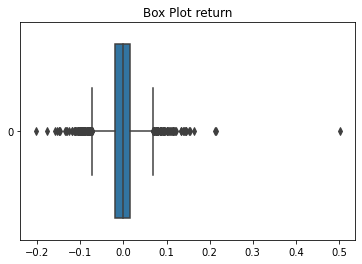
\includegraphics[width=.9\linewidth]{Images/Box Plot of Return.png}
    \caption{Box plot of log-return}
    \label{log return box}
\end{subfigure}%
\begin{subfigure}{.5\textwidth}
    \centering
    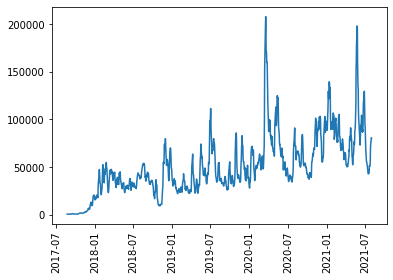
\includegraphics[width=.9\linewidth]{Images/Volume Rolling Average.png}
    \caption{7 day rolling average of the volume}
    \label{7day rolling volume}
\end{subfigure}
\caption{(a) Box plot of log-return of BTC in the given period. (b) Line plot of the rolling average of the volume.}
\label{fig:test}
\end{figure}

\subsection{Average hourly BTC/USDT log-return by day, by week, and by month}

This data is important to consider to get an overarching appreciation of how prices changes according to time -- a historically pivtoal factor in the trading of financial products. For example, one major difference between traditional stock markets and cryptocurrency markets is activity of weekends, which is not present in the former, and so behaviour at the open and close of the trading week needed to be considered carefully. In this field, the markets never sleep and so we expect to find somewhat different, interesting behaviours.
From the visualisations inf Figures (\ref{Average hourly log-return for BTCUSDT per day} - \ref{Average hourly log-return for BTCUSDT per month}) we find that historically, Thursday is a bad trading day, subsequently if we ever use historical trends as an indication of future trends, we may want to consider avoiding trading on this particular day. Similarly, we see that the months of March and September are historically quite bad months to trade and we may want (assuming this trend will repeat in the future) to sell our BTC assets in the beginning of these months and buy back at the end of these months.
\begin{figure}[!htbp]
    \centering
    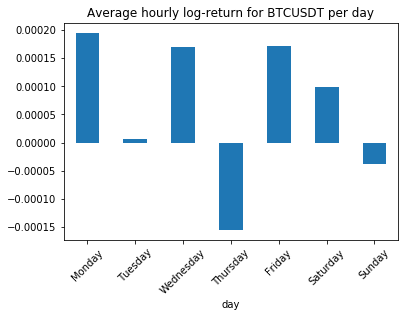
\includegraphics[width=0.7\linewidth]{Images/Average hourly log-return for BTCUSDT per day.png}
    \caption{Average hourly log-return for BTCUSDT per day}
    \label{Average hourly log-return for BTCUSDT per day}
\end{figure}

\begin{figure}[!htbp]
    \centering
    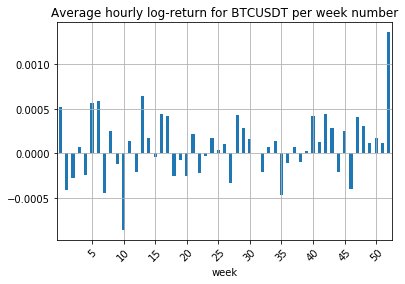
\includegraphics[width=0.7\linewidth]{Images/Average hourly log-return for BTCUSDT per week number.png}
    \caption{Average hourly log-return for BTCUSDT per week number}
    \label{Average hourly log-return for BTCUSDT per week number}
\end{figure}

\begin{figure}[!htbp]
    \centering
    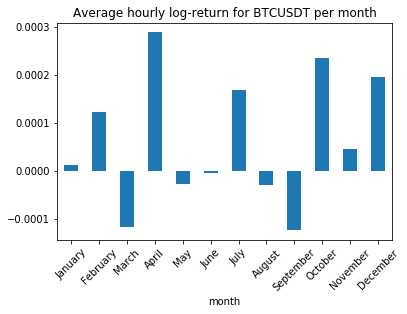
\includegraphics[width=0.7\linewidth]{Images/Average hourly log-return for BTCUSDT per month.png}
    \caption{Average hourly log-return for BTCUSDT per month}
    \label{Average hourly log-return for BTCUSDT per month}
\end{figure}








\chapter{Social media's influence on cryptocurrency prices}

Unlike the traditional stock market, cryptocurrencies are traded without many regulations and are accessible to essentially anyone with an internet connection. Therefore it is not surprising that cryptocurrencies are perhaps more sensitive to human behaviour than traditional stocks; including a much more chaotic response to sudden trends and attitudes of these traders. This is indubitably heavily impacted by social media. We aim in this chapter to leverage this observation to generate winning strategies for trading on the market. Once a strategy has been constructed, it is then tested using a so-called \textbf{backtesting} algorithm. This term indicates that our strategy is applied to historical data to assess its performance over already observed prices.  

\section{Youtube trends}\label{YT Trends}

Youtube is the most dominant streaming platform worldwide. Many Youtube channles concentrate their content solely on cryptocurrencies, consequently we find that sometimes they impact small market cap cryptocurrencies. In general, low market cap cryptocurrencies (below $10
$M USD) historical prices and data are hard to access and each require APIs from numerous cryptocurrency exchanges. Therefore, we will confine ourselves here to a general trend analysis of popular crypto Youtube channels.
First we seek to figure out the search trends of Youtube, using Pytrends, an API for Google Trends, which allows us to retrieve the trending on Google search engines, including Youtube. We get the most trending queries on Youtube for the word 'Cryptocurrency'. From these we see four popular cryptocurrencies channel stand out, namely: Bitboy Crypto, Banter Crypto, Jrny Crypto, and Crypto Zombie. Figures (\ref{youtube_channel_crypto_trends}-\ref{countries_map_2}) visualises the interest over time and geography in each of these channels.

\begin{figure}[!htbp]
    \centering
    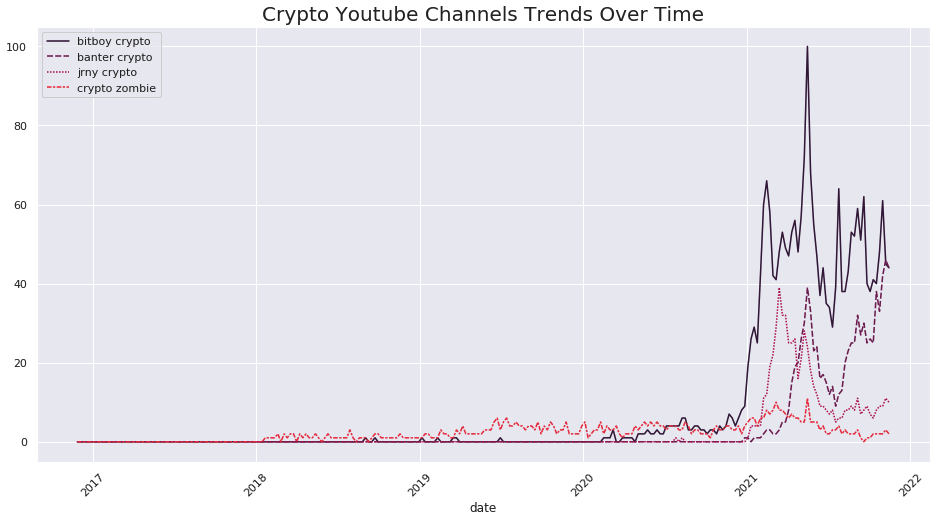
\includegraphics[scale = 0.5]{Images/youtube_channel_crypto_trends.png}
    \caption{Bitboy Crypto charges 60k USD to publish a video on upcoming cryptocurrencies, as per his notoriety.}
    \label{youtube_channel_crypto_trends}
\end{figure}

\begin{figure}[!htbp]
    \centering
    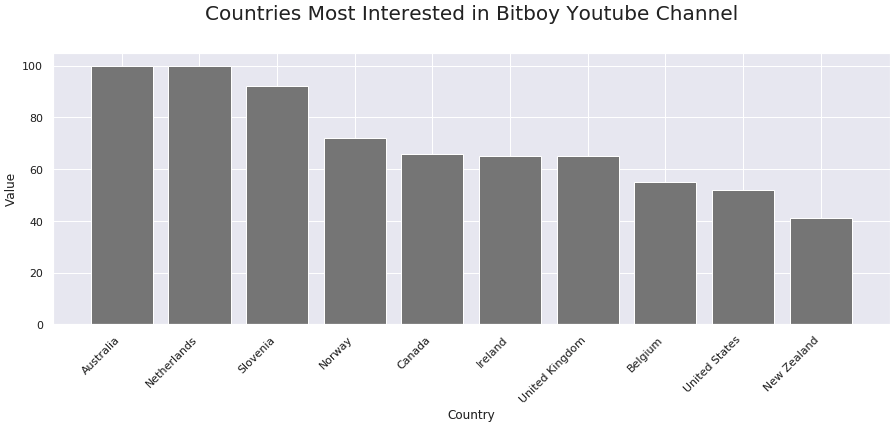
\includegraphics[scale = 0.5]{Images/countries_rank_bitboy_crypto_youtube.png}
    \caption{Bitboy Crypto is unsuprisingly most trending in anglophone countries. The \code{Choropleth} map provided by \text{Folium} python package is used to generate this plot.}
    \label{countries_rank_bitboy_crypto_youtube}
\end{figure}

\begin{figure}[!htbp]
    \centering
    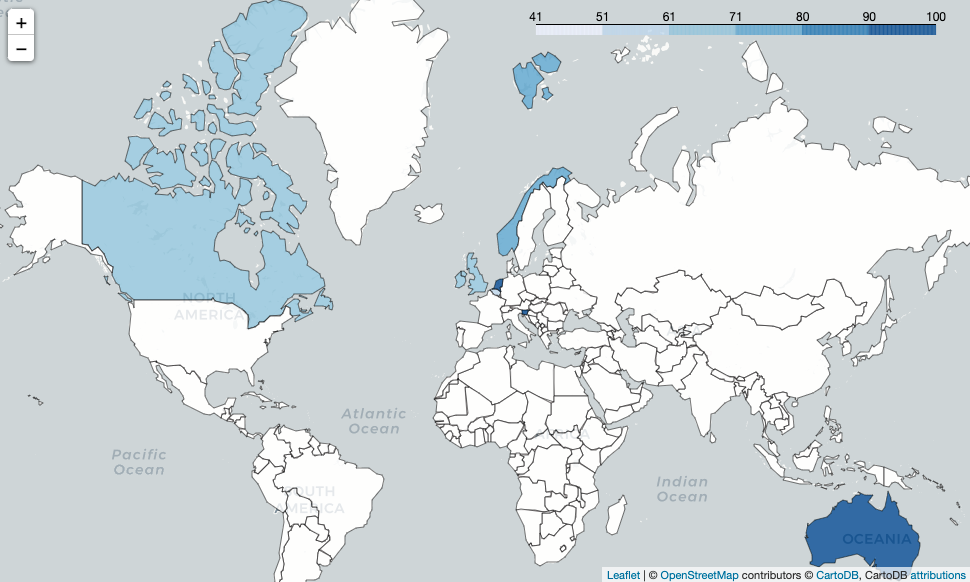
\includegraphics[scale = 0.4]{Images/countries_map_2.png}
    \caption{Map of the countries most trending for the Youtube channel Bitboy Crypto}
    \label{countries_map_2}
\end{figure}


\section{Twitter}
Twitter is an American microblogging and social networking service on which users post and interact with messages known as "tweets". Users can post, like, and share (or retweet) tweets. Millions of people from a wide variety of positions and backgrounds react and share their opinions on the platform. This includes people of great significance  and influence within society, for example the former president of the US, Donald Trump, used Twitter extensively to communicate with the American citizens during his mandate.

One finds that some individuals are very aware of the impact they have on social media and often use their influence unreservedly. Elon Musk, a very well-known serial entrepreneur and founder of Tesla, who is also the richest man on the planet, has been heavily criticized for his influence on a few cryptocurrency stocks. %He has embraced his role and was proclaimed the Doge Father by the crypto community in reference to the cryptocurrency Dogecoin. He has been creating immense moves (both up and down) of price charts with his tweets.

\subsection{Twitter strategy: Elon Musk}
Elon Musk's tweets unquestionably have great power. To create great profit inducing trading strategies it serves to try and quantify the power influencers like Elon Musk possess. In this section we will explore a simple trading strategy applied to BTCUSDT and DOGEUSDT currency pairs: \begin{strategy}[Elon Musk]
Buy $1000\text{\$}$ whenever Elon musk tweets about a given cryptocurrency and hold this position for 24 hours. Once the 24 hour period has ended, sell the stock.
\end{strategy}\label{strat:musk} 
We will visualise the effectiveness of this strategy through the \textbf{profit and loss} (PnL) generated by this strategy. If our portfolio (number and type of quantities traded) has value $V_t$ for $t$ an index of time, then the sequence $(V_t)_{t=0}^T$ for some end-time $T$ is called the profit and loss of the portfolio through time.

Users interact with Twitter through browser or mobile front-end software, however in order to collect their data from that platform computationally one has to do it via Twitter's APIs in a similar way to what we did to get the data from Binance.
We have used the python library \code{snscrape.modules.twitter} to collect the data we needed. We then updated the buy signal accordingly. We have scraped Elon Musk's tweets in search of occurrences of the character strings 'BTC', 'bitcoin', 'dogecoin' or 'DOGE' to create the datasets dealing with bitcoin and dogecoin respectively. To do that we have used the function \code{sntwitter.TwitterSearchScraper}. The results are visualised in Figures (\ref{fig:elon_btc_pnl} - \ref{fig:elon_doge_pnl}).

\begin{figure}[!htbp]
    \centering
    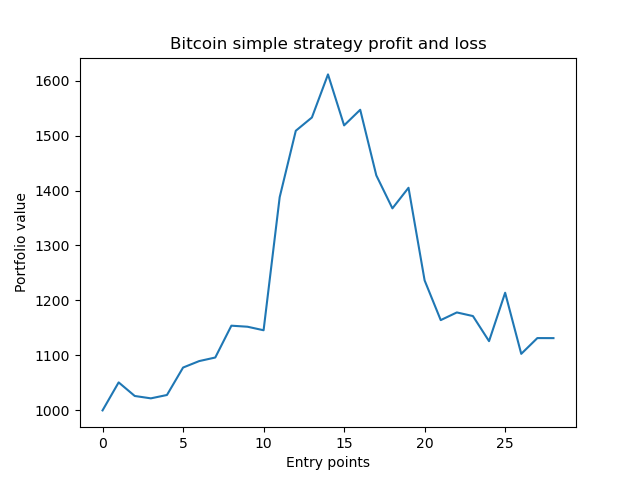
\includegraphics[scale = 0.5]{TestPlots/plot-BTC-pnl.png}
    \caption{Visualisation of PnL for a Bitcoin portfolio traded using the Elon Musk strategy. Although this strategy leads to a 20\% increase of the value of our portfolio for Bitcoin overall. We notice the presence of both a big up-trends and massive drops.}
    \label{fig:elon_btc_pnl}
\end{figure}

\begin{figure}[!htbp]
    \centering
    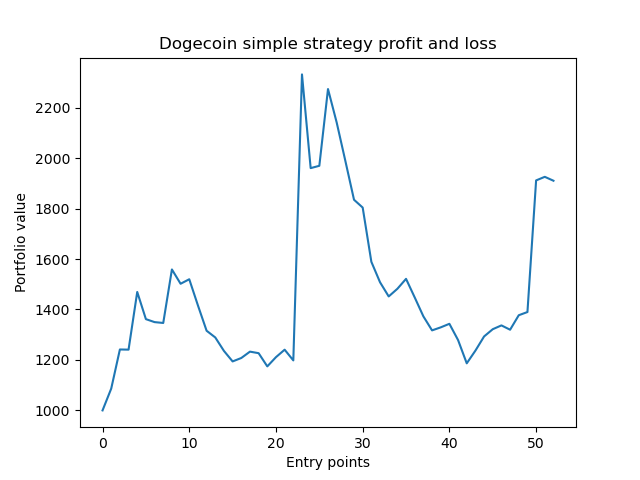
\includegraphics[scale = 0.5]{TestPlots/plot-DOGE-pnl.png}
    \caption{Visualisation of PnL for a Ethereum portfolio traded using the Elon Musk strategy. The strategy looks better for Doge and we can see a 100\% increase of the initial investment.}
    \label{fig:elon_doge_pnl}
\end{figure}
Tweets have a noticeable effect on the price of a currency, however, a tweet can negatively impact the price and suggests that one should pay attention to what is said in a tweet. For instance the huge up-trend after the $10^{th}$ entry point corresponds to a tweet in which he said "You can now buy a Tesla with Bitcoin" [24/03/2021]. We can infer that, this short sentence gave people a lot of hope and showed the interest of a massive company towards the cryptocurrency. The uptrend continued but then he talked about the risks and limitations of Bitcoin and said ``Bitcoin is actually highly centralized, with supermajority controlled by handful of big mining (aka hashing) companies. A single coal mine in Xinjiang flooded, almost killing miners, and Bitcoin hash rate dropped 35\%. Sound “decentralized” to you?" %\cite{Elon}[16/05/2021]. 
From this we can infer that Bitcoin traders lost confidence in the cryptocurrency, to use the crypto slang it spread FUD (fear uncertainty and doubt), and that caused a massive drop of the price. Knowing that a single person had so much power and could influence the prices easily in either way scared investors and Elon Musk received a lot of criticism and was accused of purposely affecting the markets to push his company's agenda. This criticism has led to a noticed dampening effect of his tweets \cite{ElonCriticism}. Following this logic, it seemed natural to try to get a sense of how optimistic a tweet was before deciding whether or not to buy. For that very reason we have chosen to use the python library \code{textblob} \cite{loria2018textblob} for processing textual data and proceed to the sentiment analysis of the tweets. The function \code{sentiment.polarity} gave a score in $ [-1,1]$ indicating how positive a text is using averaging methods. For instance : \[\code{sentiment.polarity}(``\text{good}")=0.7\;\;\;\:\:\code{sentiment.polarity}(``\text{bad}")=-0.7.\]
\vspace{-1.5em}
\begin{strategy}[Augmented Elon Musk: Adding Sentiment]
Augmented Elon Musk strategy. We add the condition that the tweet had to have a sentiment score greater or equal to $0.2$ for us to buy.\end{strategy}\label{strat:sent} 
\begin{figure}[!htbp]
    \centering
    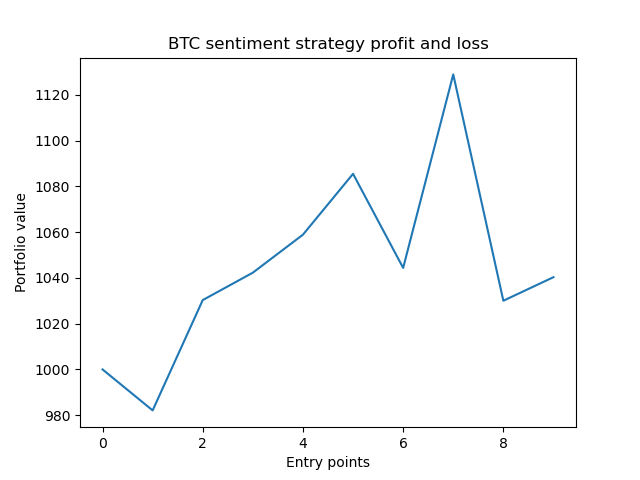
\includegraphics[scale = 0.5]{TestPlots/plot_sentiment_btc.png}
    \caption{PnL for a portfolio consisting of Bitcoin only, bought and sold according to the augmented Elon Musk strategy. The sentiment condition has missed on great upward motions as well as drops, the portfolio value still raised but only by 6\%. Which is not significant at all, especially for crypto stocks.}
    \label{fig:elon_sent_btc_pnl}
\end{figure}
\begin{figure}[!htbp]
    \centering
    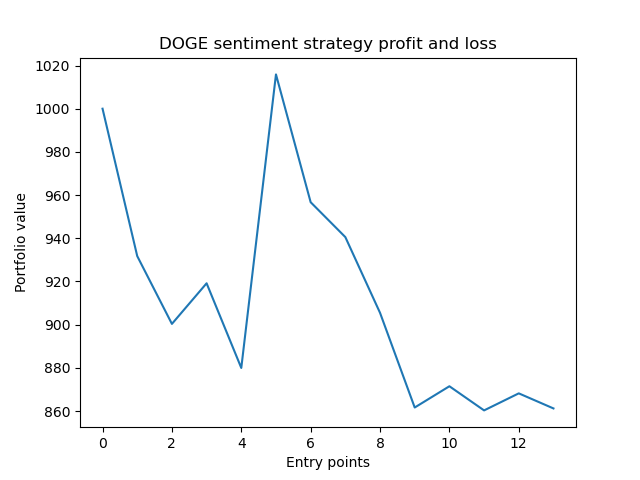
\includegraphics[scale = 0.5]{TestPlots/Doge_sentiment_plot.png}
    \caption{PnL for a portfolio consisting of Ethereum only, bought and sold according to the augmented Elon Musk strategy. The strategy is clearly not efficient for doge. We lose on our position most of the time.}
    \label{fig:elon_sent_eth_pnl}
\end{figure}

This reduced the number of entry points by more than a half but missed out on great opportunities while doing so. That is probably because neutral sentences containing crucial information can be misinterpreted by the sentiment function. Indeed the sentence "you can buy tesla with bitcoin" has a score of $0$, While the sentence "bitcoin consumes too much energy" has a score of $0.2$. Of course this is also because our person of interest, Elon Musk, is not trying to energize the public but just making an announcement. In conclusion trying to gauge the sentiment of his tweets wasn't the best approach, and resulted in a loss of capital.
Sentiment analysis is an efficient technique and should be used at a bigger scale when analyzing an important amount of tweets coming from different people, using it on a single person could lead to errors due to the personality of the source.

\subsection{Twitter strategy: Ben Armstrong informative page}
Ben Armstrong is a YouTuber, podcaster and crypto enthusiast. Better known as BitBoy Crypto, the same individual as in section \ref{YT Trends}, his objective is to educate and inform the crypto community. Indeed, his having millions of devoted followers made analysing his tweets seem relevant. Our aim is to analyse the sentiment of his tweets before investing, and find out if making decisions based on this sentiment leads to a valuable strategy. Precisely, we will comparing the profit and loss between buying blindly at every BitBoy Crpyto tweet mentioning Bitcoin and buying when signalled by a sufficiently positive BitBoy tweet. 
\begin{strategy}[Crypto-influencer]
Buy Bitcoin when a BitBoy Crypto tweet has a sentiment score above a certain threshold.  
\end{strategy}\label{strat:sent} 
\begin{figure}[!h]
\begin{minipage}{.5\linewidth}
\centering
\subfloat[]{\label{pnl:a}\hspace{-2.5em} 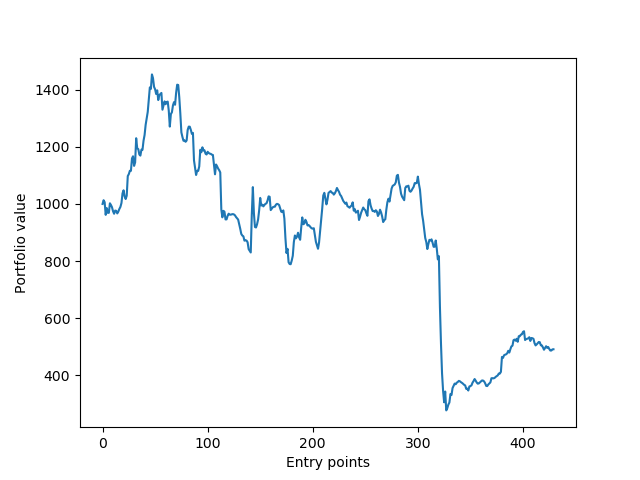
\includegraphics[scale=.6]{twitter_scraping/bitboy_pnl.png}}
\end{minipage}%
\begin{minipage}{.5\linewidth}
\centering
\subfloat[]{\label{pnl:b}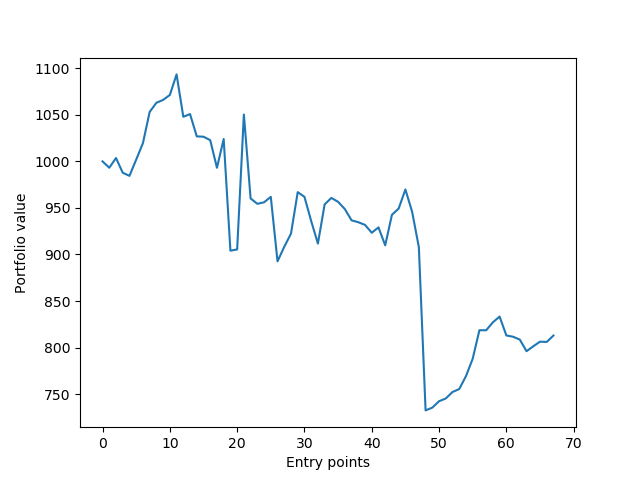
\includegraphics[scale=.6]{twitter_scraping/bitboy_pnl_sent.png}}
\end{minipage}\par\medskip
\centering
\caption{(a) Profit and loss from buying blindly after every tweet. (b) Profit and loss with sentiment threshold. Despite the fact that the number of entry has been reduced by a factor of 6, the PnL curve still has the same shape, however has experienced a negative shift (lower highs and lower lows).}
\label{fig:pnl_naji102}
\end{figure}

Analyzing the sentiment of the tweets seems to be inaccurate and doesn't give any useful results. Our method and the package used is perhaps too simplistic. More advanced natural language processing methods should be considered, using machine learning techniques to take into account the crypto jargon might give much better results. We should also remark that crypto influencers are sometimes paid to promote a certain currency therefore one should be cautious when investing with this strategy. 

%Actually shorting bitcoin at every tweet would generate profit.


\subsection{Twitter strategy: whale watching}
Indubitably, the idea of putting your money where wealthy people are putting theirs feels like a wise strategy to generate profit. A \textit{whale} is a cryptocurrency term that refers to individuals or entities that hold large amounts of a cryptocurrency. The Blockchains on which major cryptocurrencies are ran are public -- even though all users are not identifiable when an individual buys or sells a position worth millions of dollars -- so the information is available for everyone to see. It is fair to assume that the transactions of major players are aimed at moving markets in ways that benefit them at the expense of those on the other side of the trade (retail buyers) because they are trading to increase the value of their own portfolio. On twitter, there are a lot of accounts reporting such moves and a strategy could be to follow these big transactions and to buy when they happen.

Our intuition inspired us to monitor whales to see their trading patterns and to get a sense of their holdings. If whales are reducing their holdings as the price goes up, one could infer that a market peak could be approaching.
\begin{strategy}[Whale Watching]
Scrape the twitter account "WhaleTrades" looking for both the appearance of "\$ETH" and "longed" which essentially means that an important amount was bet on the rise of Ethereum, and buy when this happens. 
\end{strategy}\label{strat:sent} 

\begin{figure}[!htbp]
    \centering
    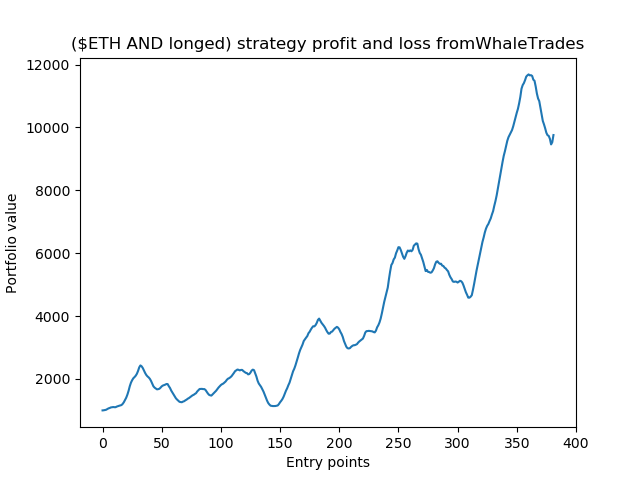
\includegraphics[scale = 0.5]{twitter_scraping/ETH-whales.png}
    \caption{Profit and loss from the whale watching strategy. Our initial investment is 12 times the the value used in previous experiments. We observe that the drops are controlled.}
    \label{fig: wwPnL}
\end{figure}

If we compare the PnL in Figure (\ref{fig: wwPnL}) to other strategies, we observe a healthy improvement here. We may take this as an indication that markets are heavily manipulated, meaning more savvy retail buyers can leverage this buy following media to make profits, while the market makers take advantage of poor decisions by layman retail buyers to continue their market manipulation strategies.

\subsection{Discussion}

\section{Medium}\label{sec:medium}
Medium is an American online publishing platform developed by Evan Williams and launched in August 2012. The platform gives its members the ability to read and participate in social journalism, having a hybrid collection of amateur and professional people and publications. The site is regularly regarded as a blog hosting platform \cite{streitfeld2017internet}.




As we know, many cryptocurrencies are run by companies or individuals. They maintain the currency they create, and they use social media to promote their cryptocurrency. Medium, as a famous and influential social media platform, is often used to promote the cryptocurrency they create. One idea we came about is that there may have some relationships between the medium and price changing of their cryptocurrency. In this section, we aim to develop strategies using the information from their medium blog. As an example, we focus on a certain cryptocurrency called Kyber (KNC). Though there are differences between each cryptocurrency, the analysis and the strategies can be applied to other cryptocurrencies as well. 



\subsection{Data Preprocessing}
Let us explain how we access the data from Medium and the changes of cryptocurrency price. For Medium publications, we use webscraping techniques via some Python libraries (\code{BeautifulSoup4 , request} and \code{selenium}). At first, we use \code{request} to acquire the source code of the website from \url{https://medium.com/@kyberteam}. This allows us to access the information via Python. Using the library \code{selenium}, we are able to acquire the full information of the source code. After that, we use functions in the library \code{BeautifulSoup4} to parse the whole source code. By doing so, we can deal with this HTML information much easier with Python. With the \code{find\_all} function, we can find all information that interests us in each article. In our case, we think the update time of the article and the title of the article might be helpful for developing strategies. Therefore, using techniques we just introduced, we have a dataframe that contains the update time (denoted as \code{date}) and title for all of the medium articles (denoted as \code{title}) from Kyber.
Upon closer inspection, we found that Kyber do not update their Medium account everyday. We guess updating an article or not is a good signal in developing strategies. So we make a new feature called \code{signal}. It is a binary variable, and the entry is given value 1 if Kyber posted on that day on Medium and 0 otherwise.  For the \code{title}, we want to apply sentiment analysis used in Twitter and keyword checking (To see if it contain certain keyword like 'announcement') at first. However, as a big company based in Asia, Kyber published a large amount of articles that not in English. As a result, it is not easy to do the analysis based on these different languages.  

We merge price data obtained from Binance with the dataframe containing information from Medium. After choosing relevant information, we have some features that are listed in the Table \ref{tab:feature}. As the Kyber begun to trade on Binance on 12 June 2020, the data we select are between 12 June 2020 and 16 November 2021, to give a current dataset. 


\begin{table}[!htp]
    \centering
    \begin{tabular}{|l|p{0.8\linewidth}|}
        \hline
        \code{date}  & Date of trading \\
        \code{high} & The highest price of the day\\
       \code{low}& The lowest price of the day\\
       \code{close} & The close price of the day\\
       \code{Open}& The open price of the day\\
         \code{signal} & Binary indicator vector of Kyber article posts indexed by day. An entry is given the value $1$ if Kyber posted on that day and $0$ otherwise.\\
         \code{opcl}  & The log difference between the open price and close price \code{$\log(close)-\log(open)$} \\
        \code{volume} & The amount of money traded at that day.\\ \hline
    \end{tabular}\vspace{2mm}
    \caption{Summary of the features from our final dataframe. On the left hand it is the feature name of data, while the right hand is the definition of them. The only feature that is obtained via the function of other features is \code{opcl}. This is an important feature for developing strategies }
    \label{tab:feature}
\end{table}


\subsubsection{Statistical Analysis}
We will investigate the strength of correlation between \code{opcl} and other features. If we find some strong correlations between \code{opcl} and some features, we can use that fact to inform a great trading price within a day. In order to do that, we use python to calculate the Pearson's correlation between them. Unfortunately, we can't find any features that strong correlate with the \code{opcl}. As can be seen from figure (\ref{medium stats}), the correlations between all the features and \code{opcl} are small. The abosolute value of them are less than 0.4, which means there is no correlations or weak correlations. Therefore, we cannot use this correlation result directly to develop a new strategy.

\begin{figure}[!htbp]
    \centering
    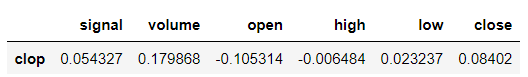
\includegraphics{Images/Medium stats.png}
    \caption{The correlation between \code{clop} and features mentioned in the features table (\ref{tab:feature}). As can be seen, all of these correlations are less than 0.4. There are no direct correlation between these features, and we can't have a direct way to develop the strategy}
    \label{medium stats}
\end{figure}


\subsection{Medium Strategy}
Besides statistical analysis, we tried some direct strategies with signals and perform backtesting to judge their usefulness. 

\begin{strategy}[Kyber Next Day]
If Kyber updates an article on date $t$, we spend all the money to buy the cryptocurrency on date $t$ with the open price and sell them all at the open price on date $t+1$.
\end{strategy}\label{strat:Kyber1}

\begin{strategy}[Kyber Same Day]
If Kyber updates an article at some time $t$, we spend all the money to buy the cryptocurrency at the open price on date $t$ and sell at the close price on date $t$.
\end{strategy}\label{strat:Kyber2} 

We compare the two strategies with a baseline, which is the simplest strategy: buy the cryptocurrency and do nothing. The value of our portfolio created this way is simply the price of the cryptocurrency over time. To perform the analysis, we assume that we have $1000$ dollars at the start of the strategy's implementation. Figure \ref{backtest medium} is the figure of price change of the two strategies and the baseline.

\begin{figure}[!h]
    \centering
    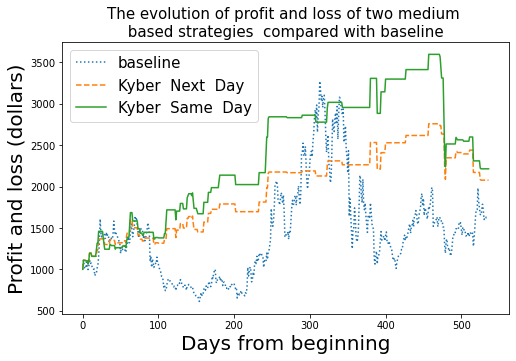
\includegraphics[scale =  0.65]{Images/medium backtesting.png}
    \caption{Backtesting of two strategies mentioned above. All the money are in USD. It can be seen clearly that the two strategy outperform the baseline the majority of the time.}
    \label{backtest medium}
\end{figure}

Clearly, the naïve do nothing strategy is sub-optimal. We see that this strategies perform very well between day 80 to day 200, where the price of Kyber drops drastically. However, they couldn't escape the big crash on day 475, and the two strategies suffer a great loss during this time. In conclusion, these two simple strategies outperform the baseline, while the second strategy performs the best.

\subsection{Discussion}

\section{Reddit}\label{reddit}
Reddit is the Internet's forum. It serves as a hub for discussion on just about anything you can think of. Naturally, therefore, cryptocurrency enthusiasts will discuss trends, advice and more in the many dedicated fora on the site such as 'r/Cryptocurrecy' or 'r/Bitcoin'. For this reason, it is not hard to imagine that there are more prominent members of the community who feature across several fora and make frequent contributions to the community. Over time, these people may gain a reputation for some type of expertise. Such people, like in the Twitter section, we will call  \textbf{influencers}. 

But how can we identify such people? Reddit is largely anonymous, and many important members of the community aren't as easily identifiable as Elon Musk. Therefore, it is important to not treat this question subjectively, since that could lead to the omission of potentially important authors whose contributions to the network of crypto traders have been valued. Consequently, we make a superficial\footnote{due to time constraints} use of network science to locate these users. 

\subsection{Reddit as a social network}\label{sec:redditSN}

Reddit, by definition, is a social network. It connects human beings together through online interaction. Therefore it lends itself to being represented mathematically in this way. However, there are many ways to do this. To list some examples, one could form: a network of fora which share users; a network of users and those who comment on their posts or a network of fora and their users. Each of these cases present distinct sets of network elements: the first, a set of fora; the second, a set of users while the third is an interesting mélange of the two. 

To illustrate the sheer versatility of this approach, and introduce some of the ideas used in our analysis, we begin by forming several networks (or interchangeably, \textit{graphs}) based on subreddits and users centered at the \textbf{r/CryptoCurrency} subreddit. The data were accessed using the extensive \code{praw} library in Python, which is used for webscraping essentially all publicly visible Reddit data. 

Before we begin, let us define some terminology that will be used throughout this section. A \textit{subreddit} is a forum dedicated to a given topic; these terms will be used interchangeably. A user, author or \textit{redditor}, is someone who actively uses reddit by making \textit{submissions} or posting \textit{comments} on those submissions, where the former are posts that start a \underline{discussion} within a subreddit. In this section, we will often work with 'top' posts. These are posts that have been identified as popular or highly rated by Reddit users. If you're not already familiar, please visit the site (\url{www.reddit.com}) and have a look around, there are myriad topics there and indubitably one will catch your eye!\\ 

We will access a set of users who have posted in the r/CryptoCurrency subreddit across the top $500$ submissions in recent history. Their activity in the subreddit is shown in Figure \ref{fig:num_posts_r_crypto}. 

\begin{figure}
    \centering
    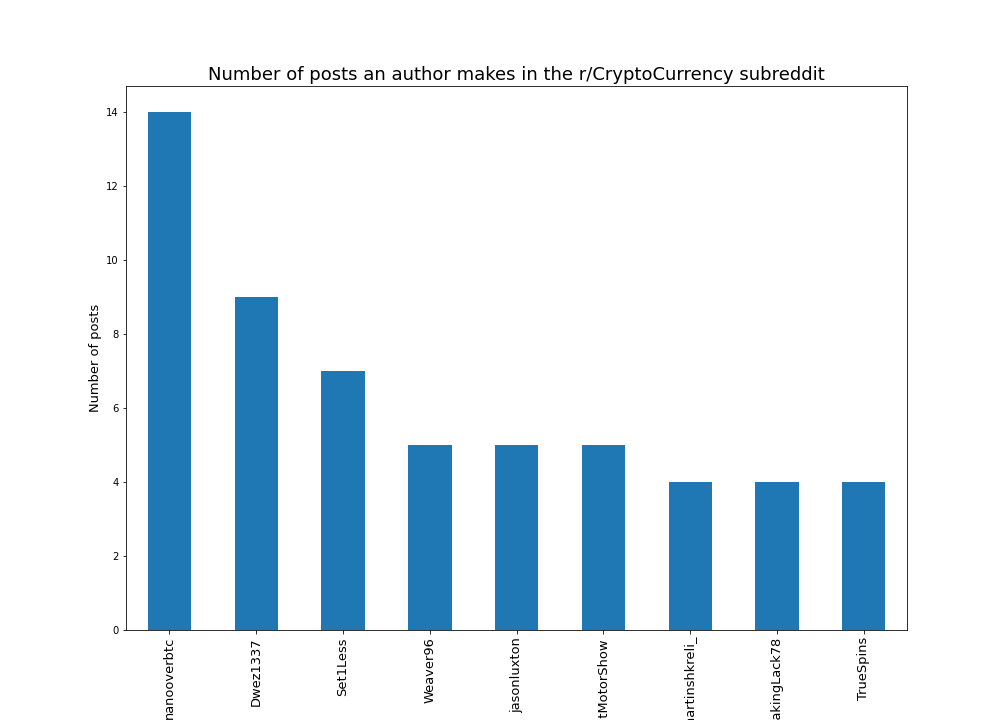
\includegraphics[width=0.8\linewidth]{Reddit_Analysis/Network_Analysis/num_posts_r_crypto.png}
    \caption{The number of posts an author makes in the r/CryptoCurrency subreddit. Notice that the names of the authors do not identify actual people, they are just online handles. This anonymity means that a truly objective approach need be taken to discover influential members of the community, before their impact is analysed.}
    \label{fig:num_posts_r_crypto}
\end{figure}

\begin{figure}
    \centering
    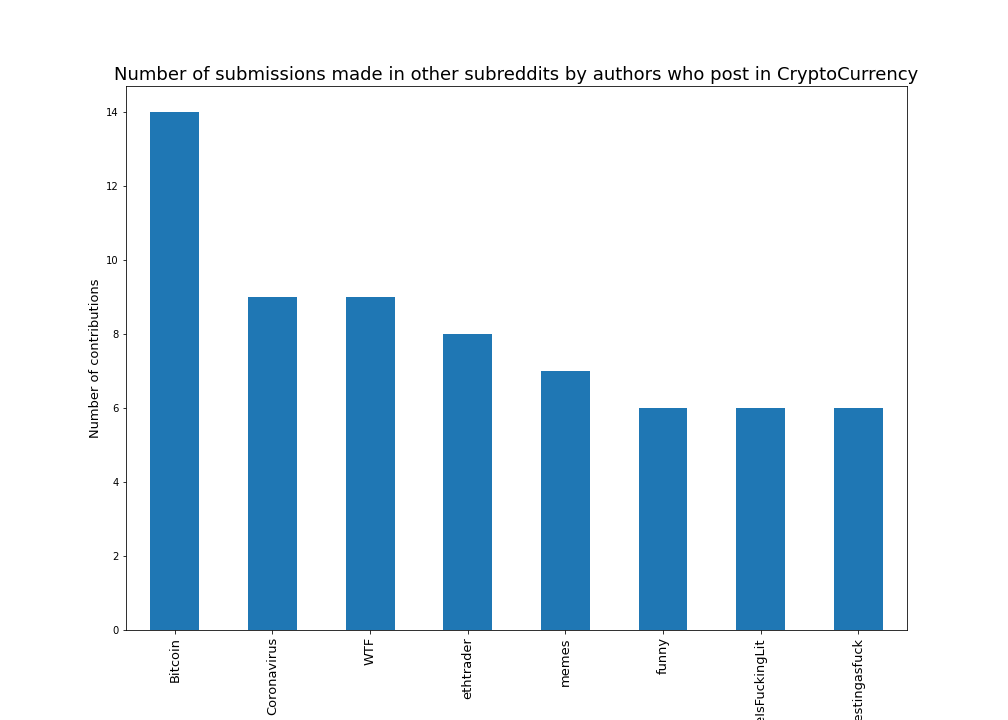
\includegraphics[width=0.8\linewidth]{Reddit_Analysis/Network_Analysis/other_subs_contributions.png}
    \caption{The other subreddits frequented by users of the r/CryptoCurrency subreddit have underlying themes. Notice that r/Bitcoin, r/ethtrader, and r/investing are some of the most discussed by users of r/CryptoCurrency.}
    \label{fig:other_subs_contributions}
\end{figure}

%\begin{figure}
 %   \centering
  %  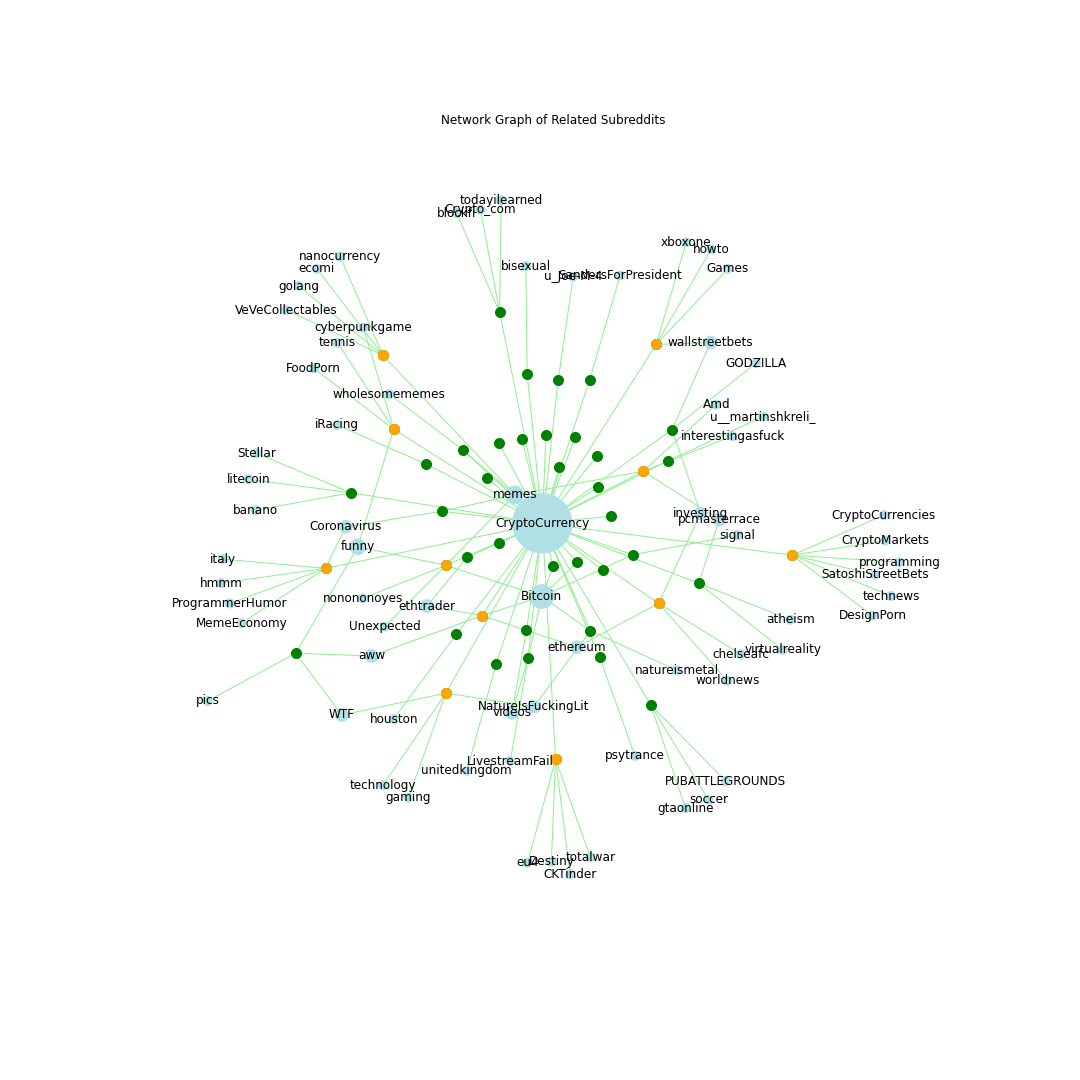
\includegraphics[scale=.525]{Reddit_Analysis/Network_Analysis/Network Graph of Related Subreddits.png}
  %  \caption{Caption}
  %  \label{fig:my_label}
%\end{figure}


Our goal for the moment is exploratory and we will investigate several properties of the users and related subreddits of r/CryptoCurrency. In this context, what do we mean by related? Here, we will also identify the subreddits in which the top authors in r/CryptoCurrency are also active, see Figure \ref{fig:other_subs_contributions} for a vusualisation. It is no surprise that subreddits like r/Bitcoin and r/ethtrader appear, while we also see that r/memes is popular as it is a general, fun forum.

To analyse this structure more deeply, we create a network, $G$, connecting these authors and subreddits. To do this, we used the extensive \code{networkX} library in Python, which has extensive documentation describing all its capabilities. The network is formed in the following way: if redditor $r$ posts in subreddit $s$, then we connect $r$ and $s$ by a \textbf{link}, which we may denote $r \sim s$ (read as: $r$ is linked to $s$). We say that the \textbf{nodes} of this network are the elements connected via a link. One should notice that a network constructed in this way has a special property. It is possible to separate the set of nodes $V$ of $G$ into two disjoint groups or \textbf{categories} $R$ and $S$ where there exist no links between pairs of nodes where each node belongs to the same set: such networks are called \textbf{bipartite}.

The substructures of networks of this type are often of interest to analysts; indeed, bipartite networks admit two \textit{projections} which reveal the underlying structure. For example, we can form a network between subreddits, $s, s' \in S$, where $s \sim s'$ whenever there is an $r$ such that $r \sim s$ and $r\sim s'$. In words: if a redditor has posted in both subreddits $s$ and $s'$, then we can create an edge between them, producing the graphs in Figure \ref{fig:bipartite}.

What can we learn from the projections? Later in this section, our goal will be to find nodes which are considered to be important or influential within a network. As a result we need a method to assign some degree of importance or \textbf{centrality} to the nodes (or links). Some measures of centrality are detailed in Table \ref{table:centralityMeasures}. To understand the need for this variety in measures imagine the following scenario: you are studying transatlantic internet traffic and its router network. The idea here is that even while the most naive measure of importance of a node, its \textbf{degree} (number of links the node has), might not be very large, it may have important positioning in the network. Routers connecting the US and the UK will be very important to this network and will separate two \textbf{communities}, even if in those communities their degree is not as high as elsewhere. It is these nodes one might wish to identify (using betweenness centrality, for example) - they are important relative to the context of the network.


\begin{table}[h]
\small
\centering
\begin{tabular}{|l|p{0.65\linewidth}|}
\hline
\multicolumn{1}{|c|}{\textbf{Centrality Measure}} & \multicolumn{1}{c|}{\textbf{Qualitative Description}}
\tabularnewline \hline
      Degree centrality & Caclulates the fraction of nodes the node of interest is connected to. It is used to determine what nodes are most connected to the rest of the network. \\
      \hline
      Betweenness  centrality & Measures the number of shortest paths that the node lies on. This centrality is usually used to determine the flow of information through the graph.\\
      \hline 
      Eigenvector centrality & Measures the node’s relative influence in the network, or how well a node is connected to other highly connected nodes. \\
      \hline 
      Edge betweenness centrality & Ranks edges by the number of shortest paths passing through the edge, similar to betweenness centrality but for edges.
 \tabularnewline \hline
\end{tabular}
\caption{Some centrality measures for nodes and edges and their descriptions.}
\label{table:centralityMeasures}   
\vspace{-4mm}
\end{table}

\begin{figure}
    \centering
    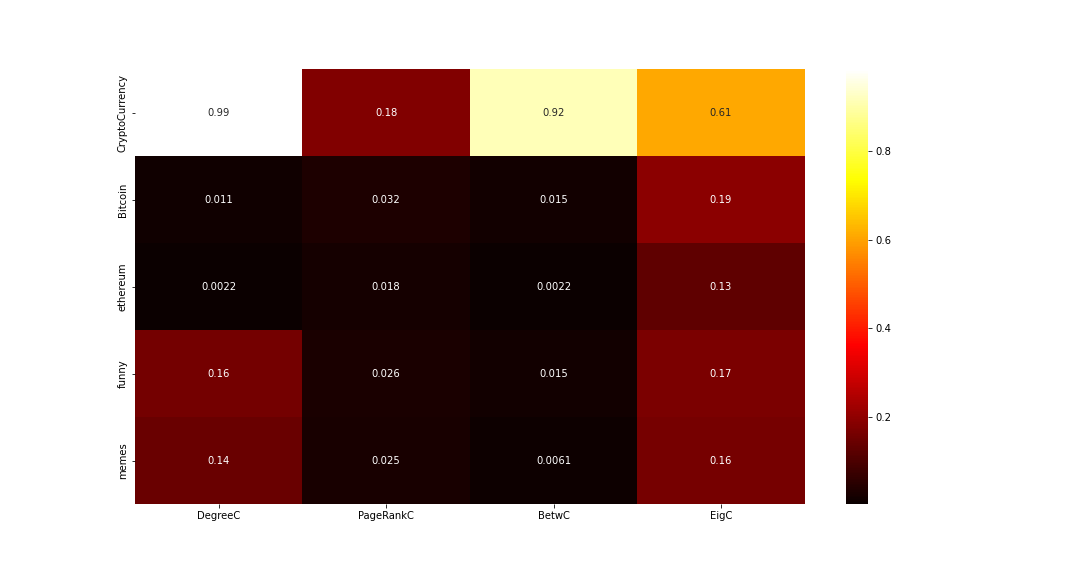
\includegraphics[width=\linewidth]{Reddit_Analysis/Network_Analysis/centrality_heatmap.png}
    \captionof{figure}{Various centrality scores for the subreddit projection $G_S$ of our original network $G$ in a heatmap, note the scores have been normalised across the graph to sum to one for each measure. We see that of course CryptoCurrency has the highest degree centrality because every redditor we considered in this section is a contributor there. However, for other measures, like eigenvector centrality, we see that the other subreddits listed here have relatively high scores considering the centrality of Cryptocurrency, and so are frequented a lot by redditors, comparatively speaking.}
    \label{fig:centralitySubreddits}  
\end{figure}




\subsection{Reddit strategy}\label{sec:redditPNL}
\begin{figure}[h]
\begin{minipage}{.5\linewidth}
\centering
\subfloat[]{\label{pnl:a}\hspace{-2.5em} 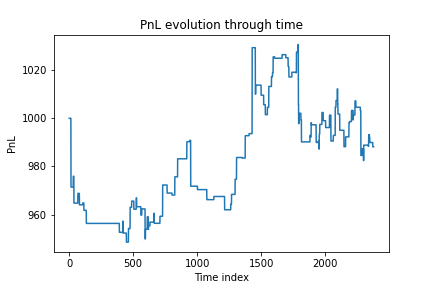
\includegraphics[scale=.6]{Reddit_Analysis/Network_Analysis/pnl_hr_naji102.png}}
\end{minipage}%
\begin{minipage}{.5\linewidth}
\centering
\subfloat[]{\label{pnl:b}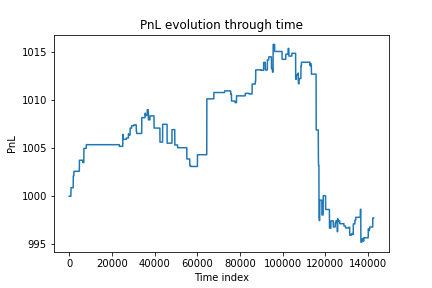
\includegraphics[scale=.6]{Reddit_Analysis/Network_Analysis/pnl_m_naji102.png}}
\end{minipage}\par\medskip
\centering
\subfloat[]{\label{pnl:c}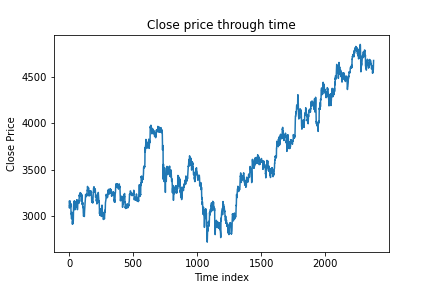
\includegraphics[scale=.65]{Reddit_Analysis/Network_Analysis/close_price_through_time_hr.png}}
\caption{(a) Profit and loss as a function of time in hours. (b) Profit and loss as a function of time in minutes. (c) The hourly close price for ethereum. All prices are in USD.}
\label{fig:pnl_naji102}
\end{figure}
We now use the ideas presented in section \ref{sec:redditSN} to identify the most influential reddit authors present in $n=24$ popular subreddits. We begin by constructing an author--commenter network, where we form a \textbf{directed} graph such that if redditor $r$ comments on a post of redditor $r'$ then $r \rightarrow r'$. Indeed, we encode now each link with a direction, hence the term \textbf{directed} network. We achieved this via the \code{praw} library by extracting the top $~400$ posts in the cryptocurrency related subreddits combined with their author and comment data. 



To study and visualise the graph, we explored the R packages \code{igraph} (the cousin of \code{networkX} in R), \code{ggraph}, \code{visNetwork}, \code{graphlayouts} extensively. Moreover, a very recent development in the field of network science has constructed the centrality measure, \textbf{Integrated Value of Influence} (IVI), which uses various statistical tests to compare various centrality measures for a graph to determine the most influential nodes \cite{IVIpatterns}. Fortunately, the authors of that paper have created a comprehensive R package called \code{influential} whose function \code{ivi} does the heavy lifting for us \cite{IVIvignette}. This function will calculate the various centrality measures for us, compute the IVI for each node, which is scaled to lie between $0$ and $100$. To explore our results, please visit our Rshiny application \textbf{\url{https://kcvis.shinyapps.io/network_analysis/}} to play around interactively with the network formed and discover properties of its nodes. 



As you see from the RShiny application, the author with the highest IVI centrality is \code{naji\_102} and a further application of \code{praw} functionality shows that the majority of their posts occur in ethereum related subreddits, so we focus on the pairing ETHUSDT for this redditor. The analysis thence effectuated consisted of applying the following strategy (in Python) to the posts of this redditor between Aug 8 and Nov 11 of 2021\footnote{The reason for this choice is computational; we extracted as many popular posts as the webscraper \code{praw} would permit --- it limits use so that their servers are not overrun.}: \begin{strategy}[Reddit influencer]
\label{PnLgeneralstrat}
If in a given time-frame, our entity-of-interest (e.g. person or news agency) outputs content on a media outlet, then the trader buys $1$ ETH at the current price and sells at the end of the time-frame. The time frame could be one second, for example. 
\end{strategy}
We do this twice: once by measuring posts by hour, and again but by measuring posts by minute, then we compare the results. The nature of the strategy produces a step-like trajectory in each case, as observed in Figure \ref{fig:pnl_naji102}. We can see that the two strategies exhibit quite different behaviours over the identical time period.




To compare their performance, we study their distribution. Plotting histograms of the data, we observe that the data for hourly and minute-wise data are bimodal and trimodal respectively, with gaussian-resembling shapes. Therefore, to draw some conclusions from the model we fit a gaussian mixture to each set of PnL data of the form \[
\sum_{j=1}^N \lambda_{i,j}\phi(x;\,\mu_{i,j},\, \sigma_{i,j})
\]
for $(i,N) \in {(h,2), (m,3)}$, where if $h$ and $m$ denote hourly and minute-wise data respectively. As standard, $\phi$ is a gaussian density. Moreover the weights (or probabilities) \[
\sum_{j=1}^N \lambda_{i,j} = 1
\]
for each $i$ and each $\lambda_{()}$ belongs to the unit interval.

\begin{figure}
    \centering
    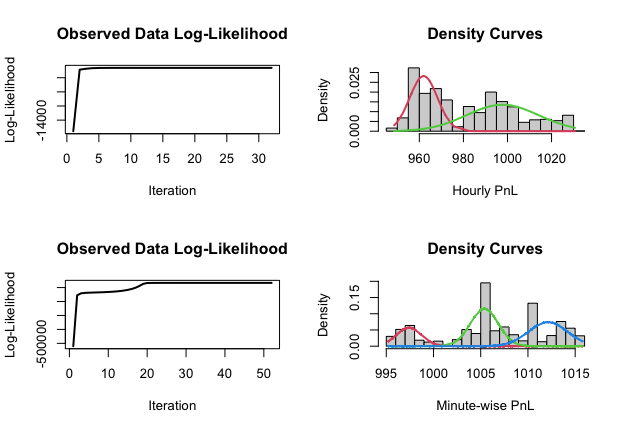
\includegraphics[width=\linewidth]{Reddit_Analysis/Network_Analysis/mixture_model_fitting.png}
    \caption{Some fitting diagnostics for the mixture model. The underlying histograms of the data are shown in grey on the right. Indeed we begin to see the log-likelihood converge after just a few iterations in the EM algorithm process. The coloured densities are the components of the mixture - they seem to capture the data well.}
    \label{fig:mixture_model_fitting}
\end{figure}

R has a package \code{mixtools} which contains a function \code{normalmixEM} which computes the parameter estimation for a given parameter $k$ number of gaussians in the mixture. The results of this estimation are given in Tables \ref{table:paramesthr} and \ref{table:paramestmin} and some diagnostics in Figure \ref{fig:mixture_model_fitting}. To estimate the uncertainty, confidence intervals for the parameters were found through bootstrapping, since this is the simplest way to derive confidence intervals for various quantities in the quite invovled EM algorithm and it is equally as informative, we performed this calculation manually in R.

\begin{table}[!htbp] \centering 
\begin{tabular}{@{\extracolsep{5pt}} ccc} 
\\[-1.8ex]\hline 
\hline \\[-1.8ex] 
 & Component 1 & Component 2 \\ 
 \hline \\[-1.8ex]
$\lambda_h$ & 0.446 &  0.554\\
$\mu_h$   &  961.940 & 997.787\\
$\sigma_h$ &  6.313 & 16.329\\
\hline \\[-1.8ex] 
\end{tabular}
\caption{Parameter estimates for hourly data found by the EM algortihm using the \code{mixtools} package in R. We remark that the means for both components are less than $1000$, which would lead to an expected value of less than $1000$ also.}
\label{table:paramesthr}
\end{table}

\begin{table}[!htbp] \centering 
\begin{tabular}{@{\extracolsep{5pt}} cccc} 
\\[-1.8ex]\hline 
\hline \\[-1.8ex] 
 & Component 1 & Component 2 & Component 3 \\ 
\hline \\[-1.8ex] 
$\lambda_m$ & 0.190 &   0.428  &  0.383\\
$\mu_m$   &  997.403 & $1005.382$ & $1012.125$\\
$\sigma_m$  &  1.330 &   1.479  &  2.059\\
\hline \\[-1.8ex] 
\end{tabular}
\caption{Parameter estimates for minute-wise data found by the EM algorithm using the \code{mixtools} package in R. We remark that the means more strongly weighted components are more than $1000$. There is more scope for the distribution to maintain values above $1000$.}
\label{table:paramestmin}
\end{table}



Indeed, these estimates are suggestive. Firstly, for the hourly data, the mean of the fitted model is less than $1000$ ($981.80$) which gives an indication that our algorithm underperforms over this period, as we are on average at a loss, while the minute-wise data gives a more optimisitic outlook. One potential reason for this is that the minute-wise strategy acts on a higher resolution than the hourly model and so is more sensitive to changes potentially caused or augmented by the comments of the author(s) we have identified and so captures the profit making opportunities more effectively. 


\begin{table}[!htbp] \centering 
\begin{tabular}{@{\extracolsep{5pt}} ccc} 
\\[-1.8ex]\hline 
\hline \\[-1.8ex] 
 & 2.5\% & 97.5\% \\ 
\hline \\[-1.8ex] 
$\mu_{h,1}$ & $961.540$ & $997.627$ \\ 
$\mu_{h,2}$ & $961.964$ & $1026.290$ \\ 
$\sigma_{h,1}$ & $6.139$ & $22.463$ \\ 
$\sigma_{h,2}$ & $0.123$ & $16.832$ \\ 
$\lambda_h$ & $0.423$ & $0.956$ \\ 
\hline \\[-1.8ex] 
\end{tabular} 
  \caption{Confidence intervals, found by bootstrap, for estimated parameters of mixed model for hourly data.} 
  \label{confinthr} 
\end{table} 

\begin{table}[!htbp] \centering 
\begin{tabular}{@{\extracolsep{5pt}} ccc} 
\\[-1.8ex]\hline 
\hline \\[-1.8ex] 
 & 2.5\% & 97.5\% \\ 
\hline \\[-1.8ex] 
$\mu_{m,1}$ & $996.960$ & $1005.391$ \\ 
$\mu_{m,2}$ & $997.391$ & $1014.062$ \\ 
$\sigma_{m,1}$ & $0.848$ & $5.126$ \\ 
$\sigma_{m,2}$ & $0.001$ & $3.338$ \\ 
$\lambda_{m,1}$ & $0.154$ & $0.738$ \\ 
$\lambda_{m,2}$ & $0.024$ & $0.687$ \\ 
\hline \\[-1.8ex] 
\end{tabular} 
  \caption{Confidence intervals, found by bootstrap, for estimated parameters of mixed model for minute-wise data.} 
  \label{confintmin}
\vspace{-1.5em}
\end{table}


To conclude, we calculate from $1000$ samples the bootstrapped $95\%$ confidence intervals for the mean of each set of PnL data. For hourly and minute-wise data respectively they are the following: $(980.916, 982.677)$ and $(1006.420, 1006.478)$. We remark that the former does not contain the estimated mean of the distribution but the lower limit is indeed very close to it. More noticeably, the former interval does not contain $1000$, so we tend to underperform with an hourly approach.

This analysis is of course limited. For example, we didn't consider the content of the posts, and we performed the analysis of a relatively short time frame. But this is analysis is intended to be informative. Going further, we would aim to continue this analysis for various authors and various (longer) time frames to build a much more comprehensive strategy which encompasses all the information we glean from that analysis, nevertheless, what we observe here is promising, and certainly supports the use of network modelling to identify important members of communities. Moreover, in an even more precise analysis, it would serve to organise posts by words mentioned in them, then we can make decisions based on the content of posts and not their existence alone.

%{\color{red} TO ADD: some form of discussion }

\subsection{Crypto Index & Sentiment Index}
The CRIX (CRyptocurrency IndeX) was constructed by Trimborn & Härdle (2018) in order to track the entire cryptocurrency market's performance. Cryptocurrencies are taken into account as soon as they check a liquidity condition that insures the conversion of said cryptocurrency to regular currencies (Fiat).
The formula of this index is as follows:
$$\text{CRIX}=\frac{\sum_i MC_i}{\text{Divisor}}$$
Where, MC is the market cap, and the divisor depends on the current supply of each currency.\\
The idea is to build a sentiment index that will follow the progression of the CRIX to be able to predict the evolution of the market as a whole. \cite{Crix}
The sentiment index will depend on google search volumes, Reddit posts, Reddit subscriptions and tweets and is computed as follows:
$$\text{SENT}=0.499 VOL_{Google}+ 0.419VOL_{Tweets} + 0.534 VOL_{RedSub}
+ 0.539VOL_{RedCmt}$$
The data was gathered using detection of keywords and platforms like stocktwits it is a social media platform similar to Twitter, but dedicated to financial discussions where investors can express opinions on any financial assets supported by the platform. StockTwits currently
supports over 532 different cryptocurrencies.\\
At first more parameters (eg. sentiment of tweets and reddit posts) were selected but were removed to avoid over-fitting \cite{Crix}.\\

To verify the accuracy of these indexes we can check the profit and loss of strategies that rely on them. 

\begin{strategy}[CRIX]
 
\end{strategy}\label{strat:sent} 

\begin{figure}[!h]
\begin{minipage}{.5\linewidth}
\centering
\subfloat[]{\label{pnl:a}\hspace{-2.5em} \includegraphics[scale=.6]{}}
\end{minipage}%
\begin{minipage}{.5\linewidth}
\centering
\subfloat[]{\label{pnl:b}\includegraphics[scale=.6]{}
\end{minipage}\par\medskip
\centering
\caption{(a) Profit and loss from buying blindly after every tweet. (b) Profit and loss with sentiment threshold. Despite the fact that the number of entry has been reduced by a factor of 6, the PnL curve still has the same shape, however has experienced a negative shift (lower highs and lower lows).}
\label{fig:pnl_naji102}
\end{figure}


\subsection{Discussion}

\chapter{Prediction Based Methods}
\section{Causality between time series}
Bitcoin is the most popular and most traded cryptocurrency on the market right now \cite{popularCryptos}. We have seen that, both superficially and subjectively, whenever Bitcoin prices against the US dollar drop (or spike) suddenly, that other cryptocurrencies tend to follow in suit. For the purposes of trading on the market, the word 'follow' is important here -- can we make decisions in buy-sell strategies of other cryptocurrencies using knowledge of Bitcoin's price trajectory in the very recent past? 

However, we must first assess whether there is any credibility to our superficial observation. To this end, we will discuss \textbf{Granger causality} and its eponymous statistical hypothesis test. A result which corroborates our initial observation would strongly inform a trading strategy which is based on Bitcoin's influence on other coins. 
\subsection{Granger Causality}
The intuition behind Granger causality is simple. Granger causality is related to the following question: if $X$ and $Y$ are variables which evolve in time, does including $X$'s past in prediction of the future of $Y$ give more likely results than not including $X$ at all? In particular, let $y$ and $x$ be \textbf{stationary} time series. To test the null hypothesis that $x$ does not Granger-cause $y$, one first finds the proper lagged values of $y$ to include in an univariate autoregression of $y$:
\[y_t = a_0 + a_1y_{t-1} + a_2y_{t-2} + \cdots + a_my_{t-m} + \text{error}_t\]
Next, the autoregression is augmented by including lagged values of $x$:
\[y_t = a_0 + a_1y_{t-1} + a_2y_{t-2} + \cdots + a_my_{t-m} + b_px_{t-p} + \cdots + b_qx_{t-q} + \text{error}_t.\]

Now, via a statistical $F$-test, one tests the individual significance of each of the coefficients $b_i$ in the above regression statement. In the notation of the above augmented regression, $p$ and $q$ are the shortest and longest lag length respectively for which the lagged value of $x$ is significant. We say $x$ \textbf{Granger-causes} $y$ upon rejection of the hypothesis \[
H_0: b_p = \cdots = b_q = 0. 
\]
In other words, if the series $y$ is better explained by including values from series $x$, then we conclude $x$ Granger causes $y$. 
In general, Granger causality has some limitations, in that does not provide any insight on the relationship between the variable hence it is not true causality unlike \textit{cause and effect} analysis. What is more, Granger causality fails to forecast when there is an interdependency between two or more variables, and Granger causality test must be performed on stationary data \cite{GrangerCausality}.

\subsubsection{Do Bitcoin prices Granger-cause Ethereum prices?}
Before proceeding in answering this question, we must ensure that the data we use meet the requirements of the Granger causality test, in that the data are stationary. As we discussion in the introduction, data extracted from online exchanges gives absolute prices of a currency at a given time, and like traditional financial time series, this is famously non-stationary. To overcome this, we make the log-return transformation \[
\log\left(\frac{P_t}{P_{t-1}}\right), 
\]
where $P_t$ is the close price at time $t$ of a given quantity. This transformation does not mask our interpretation of the results since, by a standard first order Taylor approximation \[
100\log\left(\frac{P_t}{P_{t-1}}\right) = 100\log\left(1 + \frac{P_t - P_{t-1}}{P_{t-1}}\right) \approx 100 \times \frac{P_t - P_{t-1}}{P_{t-1}},
\]
which is just a percentage return.

Obtaining the price data as described in the introduction, and using the \code{acf} function (see Figure \ref{fig:acf_btc_eth} in base R and \code{adf.test} function in the R package \code{tseries}, we are able to convince ourselves that the Bitcoin and Ethereum series are stationary. Indeed, for both series, the \code{adf.test} function, which performs the Augmented Dickey-Fuller Test whose null hypothesis says the series is non-stationary \cite{adftest} -- we obtained $p$-values less than $1\%$, and so reject this null hypothesis. 

\begin{figure}[!htbp]
    \centering
    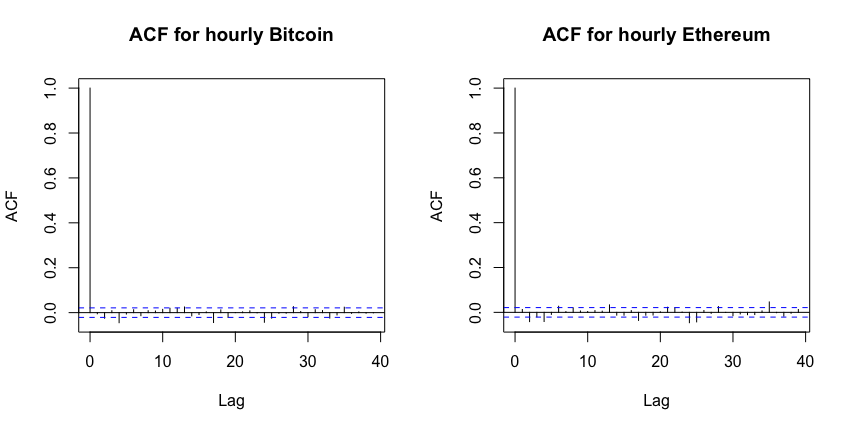
\includegraphics[width=\linewidth]{Causality_between_time_series/acf_btc_eth.png}
    \caption{Autocorrelation of the Bitcoin and Ethereum time series data respectively after a log differencing transformation. We see that it drops to zero quickly, a good indicator of stationarity.}
    \label{fig:acf_btc_eth}
\end{figure}

Having met the conditions necessary to proceed with the Granger causality test, we now employ the \code{lmtest} function in package in R containing the \code{grangertest} test function which takes the two main arguments \code{formula} and \code{order}. The former is written in the form \code{x} $\sim$ \code{y} to mean that we are test if series \code{x} Granger causes series \code{y}, and the latter specifies the size of the lag to to use. In our study, we can conveniently interpret the number of lags as the number of hours in \code{x}'s past we use to predict \code{y}, combined with \code{y}'s past. Tables \ref{tab:btc_cause_eth} and \ref{tab:eth_cause_btc} show the results, where in the former we test if Bitcoin helps in predicting Ethereum and in the latter, the reverse. We test both directions because otherwise our conclusion would be biased. 

To conclude, the results verify our intuition. Indeed, Bitcoin prices Granger-cause Ethereum prices, but \textbf{not vice-versa}. This assigns a certain degree of influence to Bitcoin price fluctuations over the prices of smaller, less traded, and less valued cryptocurrencies. While we acknowledge the Granger causality test is limited by an oversight of hidden interrelationships between other variables and the ones in consideration, given one's own experience with the markets, the conclusion remains informative.    

\begin{table}[!htbp]
\centering
\begin{tabular}{rrrrrr}
  \hline
 Lag & 1 & 2 & 3 & 4 & 5 \\ 
  $p$-value & 0.049 & 0.017 & 0.014 & 0.030 & 0.033 \\ 
   \hline
\end{tabular}
\caption{Granger causality test scores for predicting ethereum returns with Bitcoin returns. Bitcoin prices do Granger-cause Ethereum prices.} \label{tab:btc_cause_eth}
\end{table}

\begin{table}[!htbp]
\centering
\begin{tabular}{rrrrrr}
  \hline
 Lag & 1 & 2 & 3 & 4 & 5 \\ 
  $p$-value & 0.081 & 0.196 & 0.207 & 0.189 & 0.276 \\ 
   \hline
\end{tabular}
\caption{Granger causality test scores for predicting Bitcoin returns with ethereum returns. Ethereum prices do not Granger-cause Bitcoin prices.} \label{tab:eth_cause_btc}
\end{table}

\subsection{Strategy based on Bitcoin influence}

We now present a trading strategy justified by the statistical results of the previous section. We assume, guided by our observations, every time Bitcoin sees a significant drop in price, all other cryptocurrencies see significant drops in turn. \begin{strategy}[Bitcoin drops]
Whenever Bitcoin experiences a significant drop in price, we buy Ethereum, and sell in the next time period that follows.
\end{strategy} 
Note that this strategy is built on the pricnicple that more of than not,  Ethereum experiences an immediate recovery of the price once one observation sees a significant drop. However, it is entriely possible that once the price drops significantly, even more significant drops can occur immediately afterwards. To go further in our analysis, one may wish to consider moving average recovery and price retracement strategies. In Figure (\ref{fig:backtested_strategy_2}) we display the PnL ('Profit-and-Loss') of our strategy, versus a simple buy-and-hold strategy. 

\begin{figure}[!htbp]
    \centering
    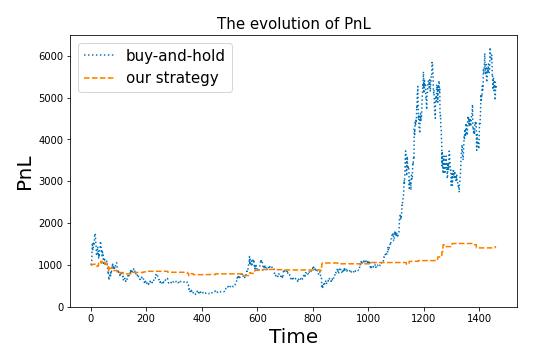
\includegraphics[width=0.8\linewidth]{Causality_between_time_series/backtested_strategy_2.png}
    \caption{Evolution of the PnL of our strategy. We observe consistent increase in our PnL eventhough it is hardly as profitable as a simple buy-and-hold strategy.}
    \label{fig:backtested_strategy_2}
\end{figure}

\subsection{Discussion}

\section{Machine Learning Approach}
Machine learning (ML) is a type of artificial intelligence (AI) that build models to become more accurate at predicting outcomes without being explicitly programmed to do so. Machine learning algorithms use historical data as input to predict new output values. Recently, machine learning performs nicely in various prediction tasks in various areas. Here we will use machine learning techniques to predict, or \textbf{forecast}, the price of cryptocurrencies.

Firstly, we introduce some statistical learning theory to do the price predictions. Statistical learning is a framework for machine learning drawing on theory from statistics and functional analysis -- its aim is to find a predictive function based on known data; it refers to a set of tools for making sense of complex dataset \cite{james2013introduction}.  











\subsection{Linear Regression and its variants}
Linear regression attempts to predict a \textbf{response variable} variable $y \in \mathbb{R}^n$ as a linear function of some known data in the form of \textbf{explanatory variables}, $\boldsymbol{x}_i \in \mathbb{R}^p$, where $i$ runs from $1$ to some integer $n$. Thus, one postulates that

\[
y= X \boldsymbol{\beta}+\boldsymbol{\varepsilon},
\]
where
\[
\begin{aligned}
X=\left(\begin{array}{cc}
1 & \mathbf{x}_{1}^{\top} \\
1 & \mathbf{x}_{2}^{\top} \\
\vdots & \vdots \\
1 & \mathbf{x}_{n}^{\top}
\end{array}\right)
\end{aligned}
\]
is called the \textbf{design matrix} for the model and $\boldsymbol{\varepsilon} \sim N(\mathbf{0}, \sigma^2 I)$, a multivariate normal vector of zero mean and independent components. This latter term embodies the error in our attempt to predict a function using a linear approach -- the data we have may only be reasonably \textit{approximated} by a linear model, we need this error term to account for discrepancies.
Now, the aim is to estimate $\boldsymbol{\beta}$. A sensible approach for this would be to find the vector $\boldsymbol{\beta}$ such that the ``error" is minimised.

\subsubsection{Ordinary least squares (OLS)}
Ordinary least squares is the most classical form of linear regression. This method aims to minimise the loss function
\[
L({\beta})= \|\boldsymbol{\varepsilon}\|=\|X {\beta}-y\|^{2},
\]
which intuitively minimises the amount of error intrinsic to the model. If  $X^{\top} X$ is invertible, or equivalently $X$ is of full rank, then the very-well known optimal solution is:
\[
{\hat{\beta}}=\left(X^{\top} X\right)^{-1} X^{\top} y.
\]
The condition that $X$ be of full rank, corresponds to a set of predictors which are largely uncorrelated. 

\subsubsection{Lasso and Ridge regression}

Ridge regression is a method of estimating the coefficients of multiple-regression models in scenarios where independent variables are highly correlated. The optimisation problem is similar to ordinary least squares but with an extra squared regularisation term, which acts to penalise the coefficients $\boldsymbol{\beta}$ to avoid overfitting when the features are well correlated. 

\[
\min _{\beta \in \mathbb{R}^{p}}\left\{\frac{1}{N}\|y-X \beta\|_{2}^{2}+\lambda\|\beta\|_{2}^{2}\right\}
\]
Again, the solution to this regularisation problem is well known
\[
\widehat{\beta}_{\text {ridge }}=\left(X^{T} X+\lambda I_{p}\right)^{-1} X^{T} y.
\]



Lasso (least absolute shrinkage and selection operator; also Lasso or LASSO) is a regression analysis method that performs both variable selection and regularization in order to enhance the prediction accuracy and interpretability of the resulting statistical model. In Lasso, we have an extra term for regularization as well. But the regularization term is first norm instead of second norm.  The optimization problem is to minimise 
\[
\min _{\boldsymbol{\beta} \in \mathbb{R}^{p}}\left\{\frac{1}{n}\|y-X \boldsymbol{\beta}\|_{2}^{2}\right\} \text { subject to }\|\boldsymbol{\beta}\|_{1} \leq t,
\]
or alternatively in the so-called Lagrangian form:
\[
\min _{\boldsymbol{\beta} \in \mathbb{R}^{p}}\left\{\frac{1}{n}\|y-X \boldsymbol{\beta}\|_{2}^{2}+\lambda\|\boldsymbol{\beta}\|_{1}\right\}.
\]
Intuitionally, the regularisation term here limits the amount of overfitting, as when $\lambda$ increases, we get more variables with zero coefficients. However, we don't have closed form solution for Lasso, and must solve the optimisation problem numerically \cite{weisberg2005applied}.



\subsection{Support Vector Machine and Random Forests}
Support vector machines and random forests were originally conceived to solve machine learning problems in \textbf{classification}, meaning the response variable is categorical. Although, they can be used in regression problems as well.

\subsubsection{Support Vector Machines}
Recall that in the ordinary least square, we try to minimize the loss function. 

\[
\min_{\boldsymbol{w} \in \mathbb{R}^{p}} \sum_{i=1}^{n}\left(y_{i}-\boldsymbol{w}^{\top} \boldsymbol{x}_{i}\right)^{2}
\]

Lasso and Ridge regression are all extensions of this simple equation, with an additional penalty parameter that aims to reduce complexity and the number of features used in the final model. Regardless, the aim — as with many models — is to reduce the error of the prediction. However, what if we are only concerned about reducing error to a certain extent? What if we don’t care how large our errors are, as long as they fall within an acceptable range? 

Enter Support Vector Regression (SVR). SVR gives us the flexibility to define how much error is acceptable in our model and will find an appropriate line (or hyperplane in higher dimensions) to fit the data. In contrast to OLS, the objective function of SVR is to minimise $L_2$ norm of the coefficient vector — not the squared error. The error term is instead handled by some imposed constraints, where we set the absolute error less than or equal to a specified margin, called the maximum error $\epsilon$ . We can tune epsilon to gain the desired accuracy of our model. Our new objective function and constraints are thus:

$$
\min _{\boldsymbol{w} \in \mathbb{R}^{p}} \sum_{i=1}^{n}\left(y_{i}-\boldsymbol{w}^{\top} \boldsymbol{x}_i\right)^{2} \quad \quad \text{subject to } \quad \quad\left|y_{i}-\boldsymbol{w}^{\top} \boldsymbol{x}_i\right| \leq \varepsilon
$$

You may quickly realize that this algorithm doesn’t work for all data points. The algorithm solved the objective function as best as possible but some of the points still fall outside the margins. As such, we need to account for the possibility of errors that are larger than $\varepsilon$. We can do this with slack variables, $\xi_i$.

\[
\min _{\boldsymbol{w} \in \mathbb{R}^{p}} \frac{1}{2}|| \boldsymbol{w}||^{2}+C \sum_{i=1}^{n}\left|\xi_{i}\right| \quad \text{subject to } \quad \left|y_{i}-w_{i} x_{i}\right| \leq \varepsilon+\left|\xi_{i}\right|
\]
Choosing great hyperparameters then solve this optimization problem is the challenge which remains \cite{noble2006support}.


\subsubsection{Random Forests}
Random Forest Regression is a supervised learning algorithm that uses ensemble learning methods for regression. In short, we train many different decision trees to do the prediction, and then we average these results to get our final model. Let us first present what is meant by a decision tree. 

A decision tree is a supervised machine learning model used to predict a target by learning decision rules from features. As the name suggests, we can think of this model as breaking down our data by making a decision based on asking a series of questions. A decision tree is constructed by recursive partitioning — starting from the root node (known as the first parent), each node can be split into left and right child nodes. These nodes can then be further split and they themselves become parent nodes of their resulting children nodes. Starting from the root, the data is split on the feature that results in the largest Information Gain (IG) (explained in more detail below). Here, our objective function is to maximize the information gain at each split, which we define as follows:


$$
I G\left(D_{p}, f\right)=I\left(D_{p}\right)-\left(\frac{N_{\text {left }}}{N_{p}} I\left(D_{\text {left }}\right)+\frac{N_{\text {right }}}{N_{p}} I\left(D_{\text {right }}\right)\right)
$$
Here, $f$ is the feature to perform the split, $Dp$, $D_{\text{left}}$, and $D_{\text{right}}$ are the data sets of the parent and child nodes, $I$ is the impurity measure, $Np$ is the total number of samples at the parent node, and $N_{\text{left}}$ and $N_{\text{right}}$ are the number of samples in the child nodes. In the regression task, the impurity measure is the weighted least squares

\[
\operatorname{MSE}(t)=\frac{1}{N_{t}} \sum_{i \in D_{t}}\left(y^{(i)}-\hat{y}_{t}\right)^{2}.
\]

In the random forest, we select different random features to build different decision trees. For predictions, we calculate the predictions for all of the decision trees and average the results in the end. This gives the result of random forest \cite{segal2004machine}.





\subsection{Feature engineering}
In order to make these statistical learning models perform as best as possible, we have to carry out a process known as feature engineering. It is the process of using domain knowledge to extract features (characteristics, properties, attributes) from raw data. The motivation is to use these extra features to improve the quality of results from a machine learning process, compared with supplying only the raw data to the machine learning process \cite{heaton2016empirical}. 
\subsubsection{Filters}
We filter the data by applying a weighting of observations across time. The
filters that will be used is the simple moving average (SMA), which weights
observations equally across a rolling time window, and the exponential moving average (EMA) which decays the weights on each observations exponentially in time \cite{brockwell2016introduction}. We regard the financial data as a signal and we use filters to extract important information.


The simple moving average applies an equal weight to all predictions within the rolling window, and is thus the average of the $m$ last days of the time series $\{X_t\}$.
\[
\operatorname{SMA}\left(\left\{X_{t}\right\}, m\right)=\frac{1}{m} \sum_{i=0}^{m-1} X_{t-i},
\]

or equivalently,

\[
\operatorname{SMA}\left(\left\{X_{t}\right\}, m\right)=\operatorname{SMA}\left(\left\{X_{t-1}\right\}, m\right)+\frac{1}{m}\left(X_{t}-X_{t-m}\right).
\]
The simple moving average weights all observations equally, even though we often consider recent observations to be more relevant. In contrast, the exponential moving average decays the weights of older observations. This can be defined recursively as

\[
\operatorname{EMA}\left(\left\{X_{t}\right\}, \alpha\right)=\left\{\begin{array}{l}
X_{0}, \text { if } t=0, \\
\alpha X_{t}+(1-\alpha) \operatorname{EMA}\left(\left\{X_{t-1}\right\}, \alpha\right), \text { if } t>0,
\end{array}\right.
\]

for any $\alpha \in [0,1]$. One common choice is $\alpha = (1+m)^{-1}$ for some $m$, which lets $m$ represents the filter's center of mass.


\subsubsection{Momentum}
Momentum is defined as the $m$ day lagged difference in closing prices:
\[
\operatorname{Momentum}\left(\left\{C_{t}\right\}, m\right)=C_{t}-C_{t-m},
\]
where $C_t$ is the close price at time $t$. This can be interpreted as an indication of trend in the time series, where positive values indicate an upwards trend in prices. For the parameter $m$, we will use values $50$, $100$ and $250$.


\subsubsection{Commodity Channel Index}
The Commodity Channel Index (CCI) is defined by:
\[
X_{t}=\frac{C_{t}+H_{t}+L_{t}}{3},
\]

\[
C C I(m)=\frac{X_{t}-S M A\left(\left\{X_{t}\right\}, m\right)}{S M A\left(\left\{\left|X_{t}-S M A\left(\left\{X_{t}\right\}, m\right)\right|\right\}, m\right)}
\]
Here, $H_t$ is the highest price of a certain period, $L_t$ is the lowest price of a certain period.  For the parameter $m$, we use $50, 100$ and $250$ days.

\subsubsection{Exponential Moving Average}
The Exponential Moving Average feature (EMAF) is defined here as the
difference of two exponential moving averages over normalized closing prices,
with different lag. Thus, it is defined as:

\[
E M A F\left(\left\{C_{t}\right\}, m, n\right)=E M A\left(\left\{C_{t}\right\}, m\right)-E M A\left(\left\{C_{t}\right\}, n\right),
\]
where m < n. The values for (m, n) are set as (30, 100),(50, 200) and (50, 250).


\subsubsection{Relative Strength Index}
The Relative Strength Index (RSI) is defined using the ratio of upward movements to downward movements, using simple moving averages:

\[
\begin{aligned}
\Delta C_{t} &=C_{t}-C_{t-1}, \\
U_{t} &=\Delta C_{t} \mathbf{1}_{\Delta C_{t} \geq 0}, \\
D_{t} &=\Delta C_{t} \mathbf{1}_{\Delta C_{t}<0},
\end{aligned}
\]

where $\mathbf{1}_{\Delta C_{t} \geq 0}$ equals $1$ if the return is non-negative, and $0$ otherwise. Using this, the RSI is defined as:
\[
R S I(m)=1-\frac{1}{1+\frac{S M A\left(\left\{U_{t}\right\}, m\right)}{S M A\left(\left\{D_{t}\right\}, m\right)}}
\]
As for the value of $m$, we again use $50, 100$ and $250$ days.

Combining all of the features mentioned above, we use them for our statistical learning approach to predicting the prices. 

\subsection{LSTM}

Consider the human brain. Humans receive millions of information everyday, but most of these data are soon forgotten; what remained in this period of time is stored in \textit{short term memory}. On the other hand, we retain some knowledge for a longer period of time, stored in long term memory. Inspired by this idea, we will employ neural network model which throws away "less important" data and memorises "more important" data. We call such a model a \textbf{Long Short Term Memory} model, often abbreviated to LSTM.
% Unlike standard feedforward neural networks, LSTM has feedback connections.
More precisely, LSTM is an artificial recurrent neural network (RNN) architecture used in the field of deep learning. It can process not only single data points (such as images), but also entire sequences of data (such as speech or video). For example, LSTM is applicable to tasks such as unsegmented, connected handwriting recognition, speech recognition and anomaly detection in network traffic or intrusion detection systems.\cite{greff2016lstm}

LSTM networks are well-suited to classifying, processing and making predictions based on time series data, since there can be lags of unknown duration between important events in a time series. LSTMs were developed to deal with the vanishing gradient problem that can be encountered when training traditional RNNs. Relative insensitivity to gap length is an advantage of LSTM over RNNs, hidden Markov models and other sequence learning methods in numerous applications. In practice, a common LSTM unit is composed of a \textit{cell}, an input gate, an output gate and a forget gate. The cell remembers values over arbitrary time intervals and the three gates regulate the flow of information into and out of the cell, see Figure \ref{fig:LSTM} for a schematic.

\begin{figure}[!htbp]
    \centering
    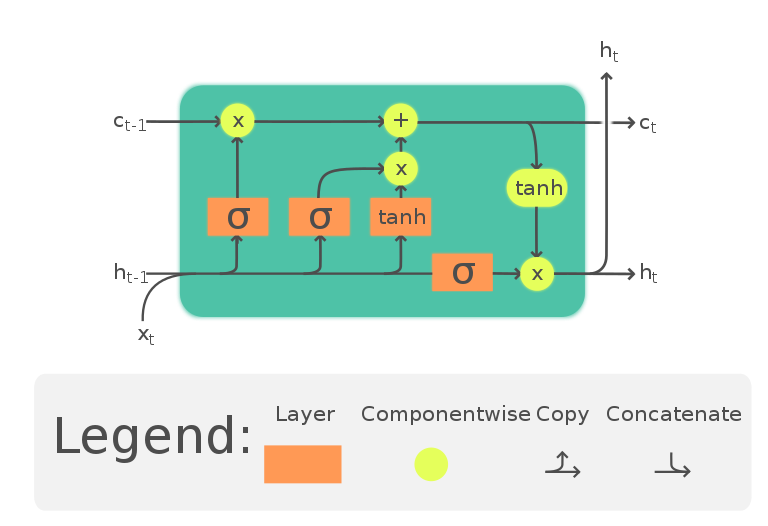
\includegraphics[scale = 0.4]{Images/LSTM.png}
    \caption{The procedure of LSTM. We update $h_t$ and $c_t$ at each iteration.}
    \label{fig:LSTM}
\end{figure}



In accordance with the Figure (\ref{fig:LSTM}), and the literature, in Table (\ref{tab:feature}) we define some of the features used in the model.
\begin{table}[!htbp]
    \centering
    \begin{tabular}{rr}
    \hline 
    \textbf{Feature} & \textbf{Description} \\
    \hline
    $ x_{t} \in \mathbb{R}^{d}$ & Input vector to the LSTM unit\\
    $f_{t} \in(0,1)^{h}$ & Forget gate's activation vector\\
    $i_{t} \in(0,1)^{h}$ & Input/update gate's activation vector\\
    $o_{t} \in(0,1)^{h}$ & Output gate's activation vector\\
    $h_{t} \in(-1,1)^{h}$ & Hidden state vector also known as output vector of the LSTM unit\\
    $\tilde{c}_{t} \in(-1,1)^{h}$ & Cell input activation vector\\ 
    $c_{t} \in \mathbb{R}^{h}$ & Cell state vector\\
    $W \in \mathbb{R}^{h \times d}$ & Weight matrices that needed to be trained\\
    $U \in \mathbb{R}^{h \times h}$ & Another weight matrices that needed to be trained \\
    $b \in \mathbb{R}^{h}$ & Bias vector parameters \\
    $\sigma_{g}$ & Sigmoid function \\
    $\sigma_{c}$ & Hyperbolic tangent function \\
    $\sigma_{h}$ & Hyperbolic tangent function or  $\sigma_{h}(x)=x$\\
    \hline 
    \end{tabular} \vspace{-0.2mm}
    \caption{Summary of the features from our final data frame. The superscripts $d$ and $h$ refer to the number of input features and number of hidden units, respectively The only feature that is obtained via the function of other features is \code{opcl}. This is an important feature for developing strategies.}
    \label{tab:my_label}
\end{table}

We define 
\[
\begin{aligned}
f_{t} &=\sigma_{g}\left(W_{f} x_{t}+U_{f} h_{t-1}+b_{f}\right) \\
i_{t} &=\sigma_{g}\left(W_{i} x_{t}+U_{i} h_{t-1}+b_{i}\right) \\
o_{t} &=\sigma_{g}\left(W_{o} x_{t}+U_{o} h_{t-1}+b_{o}\right) \\
\tilde{c}_{t} &=\sigma_{c}\left(W_{c} x_{t}+U_{c} h_{t-1}+b_{c}\right) \\
c_{t} &=f_{t} \circ c_{t-1}+i_{t} \circ \tilde{c}_{t} \\
h_{t} &=o_{t} \circ \sigma_{h}\left(c_{t}\right)
\end{aligned}
\]
where the initial values are $c_{0}=0$ and $h_{0}=0$ and the operator o denotes the Hadamard product (element-wise) product. The subscript $t$ indexes the time step. For readers that are interested in this technique, we recommend a book written by Greff on the topic \cite{greff2016lstm}.




\subsection{Prediction and Backtesting}
By applying the methods introduced in this chapter, we then developed trading strategies and assessed their performance. Firstly, we introduce the data we used and how we preprocessed them. 

The data we used to train the model is the Kyber Network trading data used in section \ref{sec:medium}. However, here the data is more granular; we use 1 hour trading data in lieu of 1 day data to train the model and test the accuracy of our model.  We split the one hour trading data into two parts. The first 80 percent of data is used as training dataset, while the remaining 20 percent data are used as testing test. For the LSTM model, we keep only two features: \code{Date} and \code{close} (log of close price in an hour). For a certain data, we use the close price of previous 60 data as input and the close price of that certain data as output. Please see section (\ref{sec:medium}) for details. For other machine learning models, we use all features we obtained from section \ref{sec:feateng}. 

%For certain data, we use the features we got above and the close price of the previous 10 data as input and the same features of that certain data as output.


In order to compare the performances of these models, we need to define a way of giving a numerical score to the the performance of our models. We will use the Root Mean Square Error (RMSE) statistic
\[\textrm{RMSE} =\sqrt{\frac{\sum_{i=1}^{N}\|y(i)-\hat{y}(i)\|^{2}}{N}},\] where $N$ is the number of data points, $y(i)$ is the i-th measurement of actual data, and $\hat{y}(i)$ is its corresponding prediction. In machine learning, it is extremely helpful to have a single number to judge a model’s performance, whether it be during training, cross-validation, or monitoring after deployment. Root mean square error is one of the most widely used measures for this. It is a proper scoring rule that is intuitive to understand and compatible with some of the most common statistical assumptions \cite{hyndman2006another}. This statistic measures the Euclidean distance between our prediction and our model, the aim is to get this figure as low as possible, offering an analogy to correctness.  

After using grid search to tune the hyperparameters, we trained a model with our training data. After obtaining the model we train, we do process the testing data and work out the prediction. In table \ref{tab:RMSE} we record the RMSE statistic obtained from these models. Figure (\ref{fig:LSTM price}) shows that the prediction obtained using LSTM deviates noticeably from the known prices, but retains the trajectory. That said, its performance is not as good as that which we obtain from OLS regression as we see that its RMSE value is smaller. Figure (\ref{fig:OLS price}) shows this prediction.
\begin{table}[]
    \centering
    \begin{tabular}{|c|c|}
    \hline
        Model & RMSE\\ \hline
         OLS Regression& 0.013         \\
         Lasso& 0.026\\
         Ridge Regression& 0.028\\
         Support Vector Machine& 0.011      \\
         Random Forest &  0.015       \\
         LSTM & 0.056\\
    \hline
    \end{tabular}
    \caption{RMSE for different models. As can be seen here, the linear SVM has the lowest RMSE, while the LSTM has the highest RMSE. These values are relatively small, which means that our predictions are close the actual prices.}
    \label{tab:RMSE}
\end{table}


\begin{figure}[!htbp]
    \centering
    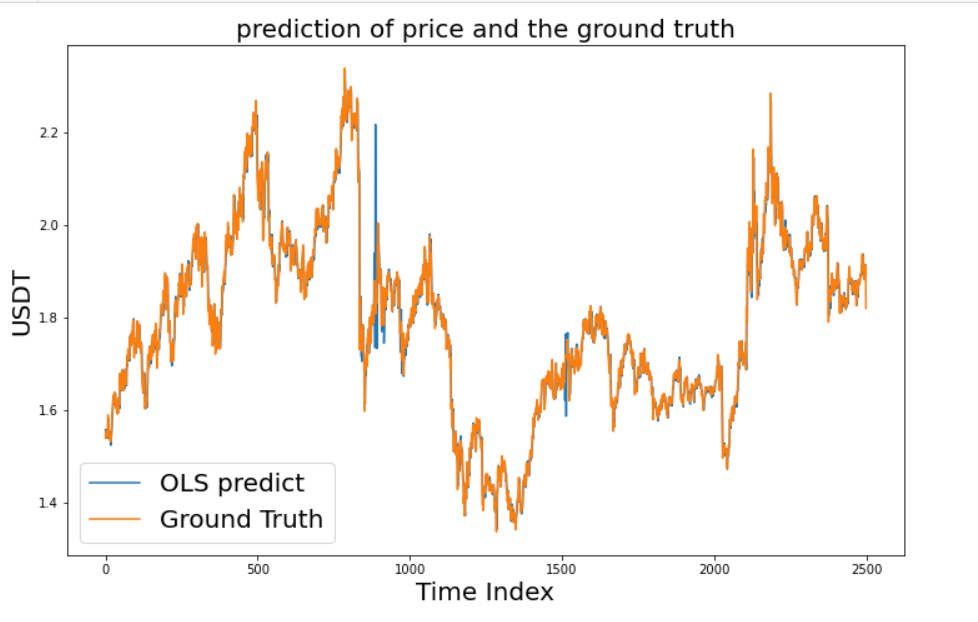
\includegraphics[scale = 0.65]{Images/OLS price prediction.png}
    \caption{Price prediction via ordinary least squares linear regression. The prediction is very close to the actual prices save for a few points.}
    \label{fig:OLS price}
\end{figure}

\begin{figure}[!htbp]
    \centering
    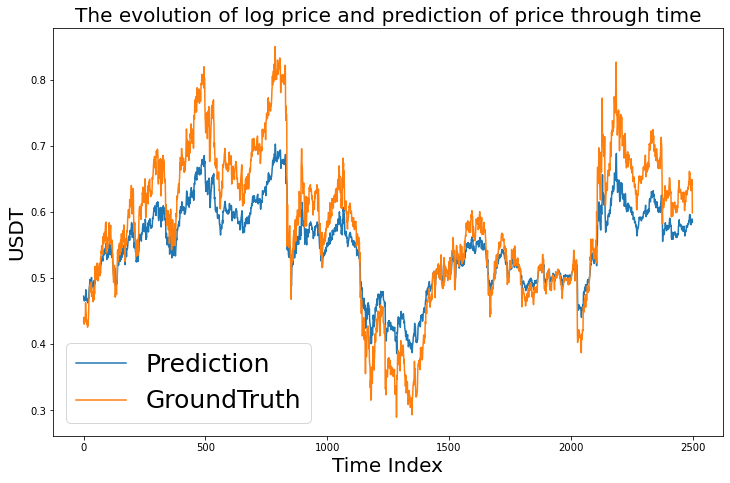
\includegraphics[scale = 0.5]{Images/LSTM price.png}
    \caption{Price prediction via LSTM. The trajectory is similar however there are more noticeable deviations from actual values.}
    \label{fig:LSTM price}
\end{figure}

\begin{strategy}[Kyber Next $s$]
This strategy is a generalisation of the Kyber Next Day strategy of section (\ref{sec:medium}). Indeed, if we predict that price at next $s$ is higher and we don't have KNC right now, then we buy the KNC. If our model predict that the price at next $s$ is lower and we have KNC right now, then we sell the price right now. In this section we set $s = \text{hour}$.
\end{strategy}

In figure \ref{fig:LSTM PNL} we display realisation of our prediction strategy via LSTM. It can be seen that our strategy works nicely and outperforms the baseline in the long run in our testing dataset. Indeed, based on the historical data we are using, our model is most accurate only during a short period of time which coincides with hours $1500-2000$. Compare this with much earlier in the data set where the prediction gives a significant underestimate. In period predicted with greater accuracy, our strategy is able to earn much money. But in the other time, our model is not much better, performs similar to the market. Overall, our strategy gives us a higher return.
\begin{figure}[!ht]
    \centering
    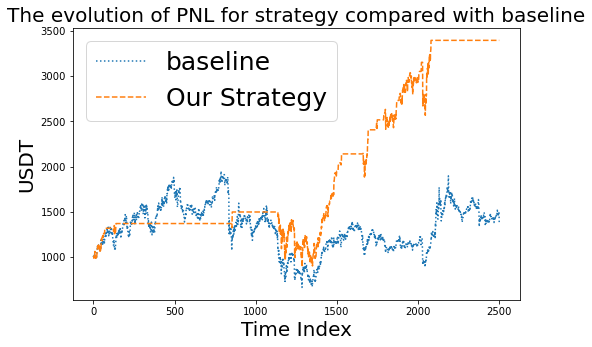
\includegraphics[scale = 0.7]{Images/LSTM PNL.png}
    \caption{PNL evolution of LSTM model and baseline. It can be seen that at beginning, our strategy perform worse than the baseline. However, our strategy performs much better during the oscillation of the KNC price.}
    \label{fig:LSTM PNL}
\end{figure}

\begin{figure}
    \centering
    
\includegraphics[scale = 0.528]{Machine Learning/PnL_regress_various.png}
    \caption{PNL evolution of our trading strategy using prediction from OLS, lasso and ridge regression models and a baseline. All models beat the baseline in the long-run.}
    \label{fig:LR PNL}
\end{figure}



\begin{figure}
    \centering
    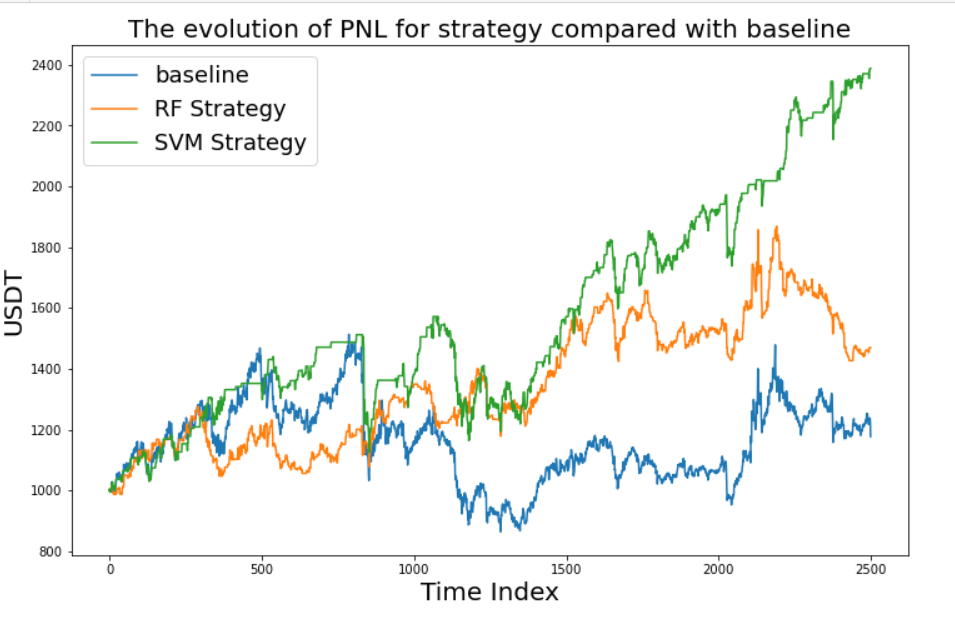
\includegraphics[scale = 0.6]{Images/PNL SVM RF.png}
    \caption{PNL evolution of random forest and SVM model. We observe better than the baseline performance again here; the SVM model shows a very healthy growth in the second half of the testing data}
    \label{fig:SVMRF PNL}
\end{figure}




\subsection{Discussion}
On the data set we used our prediction strategy, the we achieved promising returns. In figure (\ref{fig:LR PNL}) we see that all regression based methods outperform the baseline in the long run, while ridge regression has the highest return in the long-run. We also notice that even though the Lasso is worse than the baseline for a majority of time, it appears to increase for longer stretches of time than the other methods. Moreover, in figure (\ref{fig:SVMRF PNL}) we notice that the SVM method works better with the strategy than the random forest method according to the final return.\\

For all of the methods we have, they perform better than the baseline strategy and are able to generate profit. One might imagine that these PnL scores should be related to the RMSE. The smaller the RMSE is, the closer our prediction is, we guess that lower RMSE leads to a higher final return. However, we saw that the LSTM model has the largest final return while it has the largest RMSE. On the other hand, the SVM model has the lowest RMSE while it has the second largest final return. Notice that the ordinary least squares linear regression has the second smallest RMSE but has the lowest final return. Indeed, while RMSE is a useful statistic in measure the correctness of a predictive function, in the case of financial time series, the deviations at each time point play an important role in the generation of large profits and averaging them out loses this magnified view that we might desire, so as to find a relationship between the correctness of a model and its profit making abilities. 

















%\begin{thebibliography}{}
%\bibitem{medium}
 %Streitfeld, David (May 20, 2017). "'The Internet Is Broken': @ev Is Trying to Salvage It". The New York Times. ISSN 0362-4331. Archived from the original on May 21, 2017. Retrieved 2017-05-22.
%\bibitem{}



%\end{thebibliography}


\appendix
\chapter{Supplementary Figures}\label{app:supplementary figures}

\begin{figure}[h]
\begin{minipage}{.5\linewidth}
\centering
\subfloat[]{\label{birpartite:a}\hspace{-2em} \includegraphics[scale=.15]{Reddit_Analysis/Network_Analysis/author_projection.png}}
\end{minipage}%
\begin{minipage}{.5\linewidth}
\centering
\subfloat[]{\label{birpartite:b}\includegraphics[scale=.15]{Reddit_Analysis/Network_Analysis/subreddit_projection.png}}
\end{minipage}\par\medskip
\centering
\subfloat[]{\label{bipartite:c}\hspace{-2em}\includegraphics[scale=.25]{Reddit_Analysis/Network_Analysis/bipartite_demonstration.png}}
\caption{(a) Author projection of bipartite graph $G$. (b) Subreddit projection of bipartite graph $G$. (c) $G$ shown clearly with its bipartite structure. The central blue node in (b) and (c) is the r/CryptoCurrency subreddit.}
\label{fig:bipartite}
\end{figure}




\bibliographystyle{vancouver}
\bibliography{SCV_Crypto_Report(s)/references}


\end{spacing}
\end{document}

%%%%%%%%%%Maybe used later%%%%%%%%%%%%%%

%\subsection{Analysis of extremes}

\begin{figure}[!htbp]
    \centering
    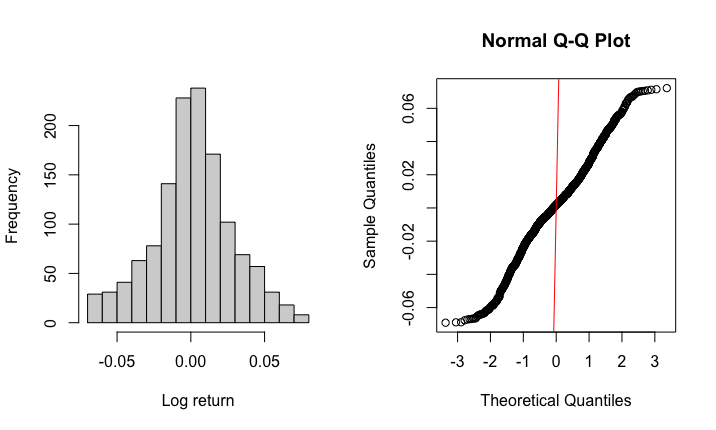
\includegraphics[width=\linewidth, scale=0.8]{Extremal Modelling/distplots_sans_outliers.png}
    \caption{Distribution of log returns having eliminated outliers and a QQ plot of the data against a standard normal random variable. Clearly the data is still heavily tailed.}
    \label{fig:distplots_sans_outliers}
\end{figure}


In finance, the question of extreme values is indubitably an important one. For example: stock market crashes, interest rates ad  insurance pricing based on life expectancy are all fields in which it would be necessary to consider rare events. The analysis of cryptocurrency trajectories is no different, indeed, sudden but large deviations in the trajectory of cryptocurrency prices would certainly be of interest to a trader. 

In light of this, it is not unnatural to ask the corresponding statistical question in the context of extremes. In Figure \ref{fig:distplots_sans_outliers}, we can see that the distribution of log returns for our data set admits very heavy tails. In this dataset there are many statistically anomalous results which skew the data, but even upon their removal, the data remain strongly skewed, see Figure \ref{fig:distplots_sans_outliers}, the data still exhibit this skewed behaviour. This sparks interest in using extreme value theory to aid our understanding of this behaviour.\\

If we observe a trajectory of prices $p_t$, for $t$ an index of time (e.g. prices per minute or hour, etc.), by assuming they come from a random sample, we can aim to fit their scaled extreme, either maximum or minimum, to a distribution of the following type \[
G(x; \eta, \tau, \xi) = \begin{cases}
\exp\left[-\left\{1+\xi(x-\eta)/\tau\right\}_+\right], & \xi \ne 0\\
\exp\left[-\exp\left\{-(x-\eta)/\tau\right\}\right], & \xi = 0,
\end{cases}
\]
where $\eta, \tau$ and $\xi$ are location, shape and scale parameters respectively. Studying maxima in this way is called the \textbf{block maxima approach}, since one groups data and considers fitting the distribution to the maxima across all groups, for example: maximum price over one day, where the prices are indexed by hours.

The goal, then, would be to fit this model to our data, i.e. by finding the unknown parameters. To this end, we have available to use the R packages $\code{evd}$ and $\code{ismev}$ which give useful functions for extremal modelling and makes plotting diagnostics straightforward. We will demonstrate their capabilities in later sections. 